% =============================================================================
%  CampusReserve - BCSE302P Database Systems Lab - Individual Mini Project Report
%  Student: Durlav Dani (24BCE2361)
%  Build:   xelatex CampusReserve_Report.tex   (run twice for contents/refs)
%  Faculty formatting: Times New Roman 12 pt, 1.5 spacing, bold 14 pt headings,
%  1 inch margins, page numbers bottom centre.
% =============================================================================
\documentclass[12pt,a4paper,oneside]{report}

% ---- EDIT THESE BEFORE SUBMITTING -------------------------------------------
\newcommand{\facultyname}{[INSERT FACULTY NAME]}
\newcommand{\submissiondate}{[INSERT SUBMISSION DATE]}
% -----------------------------------------------------------------------------

\usepackage{fontspec}
% Times New Roman if installed (Windows/macOS); otherwise TeX Gyre Termes, a
% metric-compatible Times clone shipped with TeX Live.
\IfFontExistsTF{Times New Roman}
  {\setmainfont{Times New Roman}}
  {\setmainfont{TeX Gyre Termes}}
\IfFontExistsTF{Consolas}{\setmonofont[Scale=0.88]{Consolas}}{\setmonofont[Scale=0.84]{DejaVu Sans Mono}}

\usepackage[margin=1in]{geometry}
\usepackage{setspace}
\onehalfspacing
\usepackage{graphicx}
\graphicspath{{figures/}{figures/evidence/}}
\usepackage{float}
\usepackage{booktabs,longtable,tabularx,array}
\usepackage{xcolor}
\usepackage{enumitem}
\setlist{itemsep=0.15em,topsep=0.3em}
\usepackage{listings}
\usepackage[labelfont=bf,font=small,skip=6pt]{caption}
\usepackage{titlesec}
\usepackage{tocloft}
\usepackage{fancyhdr}
\usepackage{etoolbox}
\usepackage[hidelinks]{hyperref}

% ---- Headings: bold, 14 pt -----------------------------------------------------
\titleformat{\chapter}[hang]{\fontsize{14}{17}\selectfont\bfseries}{\thechapter.}{0.6em}{}
\titlespacing*{\chapter}{0pt}{0pt}{12pt}
\titleformat{\section}{\fontsize{14}{17}\selectfont\bfseries}{\thesection}{0.6em}{}
\titleformat{\subsection}{\fontsize{12}{15}\selectfont\bfseries}{\thesubsection}{0.6em}{}
\titleformat{\subsubsection}{\fontsize{12}{15}\selectfont\bfseries\itshape}{}{0em}{}
\setcounter{secnumdepth}{2}
\setcounter{tocdepth}{2}
\renewcommand{\cfttoctitlefont}{\fontsize{14}{17}\selectfont\bfseries}
\renewcommand{\cftloftitlefont}{\fontsize{14}{17}\selectfont\bfseries}
\renewcommand{\cftlottitlefont}{\fontsize{14}{17}\selectfont\bfseries}
\renewcommand{\cftchapfont}{\bfseries}

% ---- Page numbers: bottom centre on every page ------------------------------------
\pagestyle{plain}
\fancypagestyle{plain}{\fancyhf{}\fancyfoot[C]{\thepage}\renewcommand{\headrulewidth}{0pt}}

% ---- Code listings ---------------------------------------------------------------
\definecolor{codebg}{HTML}{F5F7FA}
\definecolor{codekw}{HTML}{1F4E79}
\definecolor{codecm}{HTML}{5A6B5A}
\lstdefinelanguage{PLSQL}[]{SQL}{
  morekeywords={REPLACE,PROCEDURE,FUNCTION,PACKAGE,BODY,TRIGGER,COMPOUND,RETURN,RETURNING,IS,AS,
  BEGIN,END,DECLARE,EXCEPTION,WHEN,THEN,ELSIF,LOOP,EXIT,CURSOR,OPEN,FETCH,CLOSE,PIPELINED,PIPE,ROW,
  RAISE_APPLICATION_ERROR,PRAGMA,EXCEPTION_INIT,SYS_REFCURSOR,FOR,EACH,STATEMENT,AFTER,BEFORE,
  WAIT,SKIP,LOCKED,CURRENT,OF,NOWAIT,MERGE,USING,MATCHED,CONSTANT,TYPE,RECORD,IN,OUT,NOCOPY,
  DETERMINISTIC,ROWTYPE,NOTFOUND,ROWCOUNT,ISOPEN,SAVEPOINT,ROLLBACK,COMMIT,CHECK,CONSTRAINT,
  REFERENCES,FOREIGN,PRIMARY,KEY,UNIQUE,DEFAULT,IDENTITY,GENERATED,TIMESTAMP,INTERVAL},
  sensitive=false}
\lstset{
  basicstyle=\ttfamily\footnotesize\linespread{1.0}\selectfont,
  keywordstyle=\color{codekw}\bfseries,
  commentstyle=\color{codecm}\itshape,
  stringstyle=\color{black},
  backgroundcolor=\color{codebg},
  frame=single, rulecolor=\color{black!25}, framesep=4pt,
  breaklines=true, breakatwhitespace=false, columns=fullflexible, keepspaces=true,
  showstringspaces=false, tabsize=2, aboveskip=8pt, belowskip=8pt,
  numbers=none, captionpos=b, upquote=true,
  literate={–}{{-}}1 {—}{{--}}1 {→}{{->}}1 {≥}{{>=}}1 {…}{{...}}1 {·}{{.}}1 {’}{{'}}1 {“}{{"}}1 {”}{{"}}1 {₹}{{Rs}}2 {°}{{deg}}3
}
\renewcommand{\lstlistingname}{Listing}

% ---- Evidence placeholders ------------------------------------------------------------
% \evidence{file.png}{caption}: shows figures/evidence/file.png when it exists,
% otherwise a clearly marked grey placeholder box (never mistaken for evidence).
\newcommand{\evidence}[2]{%
  \begin{figure}[H]\centering
  \IfFileExists{figures/evidence/#1}%
    {\includegraphics[width=0.92\linewidth,height=0.42\textheight,keepaspectratio]{figures/evidence/#1}}%
    {\fcolorbox{black!45}{black!6}{\parbox[c][3.2cm][c]{0.86\linewidth}{\centering\sffamily\small
      \textbf{EVIDENCE PLACEHOLDER --- NOT YET CAPTURED}\\[4pt]
      Replace with a screenshot from your own execution.\\
      Save as \texttt{report/figures/evidence/\detokenize{#1}} and rebuild.}}}%
  \caption{#2}\end{figure}}
% \pending{...}: a measured value that has not been recorded yet.
\newcommand{\pending}[1]{\textcolor{black!55}{\textit{Pending: #1}}}

% Allow line breaks after underscores in long identifiers.
\let\origus\_
\renewcommand{\_}{\origus\allowbreak}
\setlength{\emergencystretch}{3em}

\hypersetup{pdftitle={CampusReserve - BCSE302P Mini Project Report},pdfauthor={Durlav Dani (24BCE2361)}}

\begin{document}

% =============================================================================
% 1. COVER PAGE
% =============================================================================
\begin{titlepage}
\pdfbookmark[0]{Cover Page}{cover}
\centering
\vspace*{0.6cm}
{\fontsize{24}{29}\selectfont\bfseries CAMPUSRESERVE\par}
\vspace{0.5cm}
{\fontsize{15}{20}\selectfont\bfseries Intelligent Campus Resource Booking, Maintenance \&\\ Utilisation Analytics System\par}
\vspace{1.4cm}
{\large A Mini Project Report\par}
\vspace{0.6cm}
{Submitted in partial fulfilment of the requirements for\par}
\vspace{0.3cm}
{\large\bfseries BCSE302P --- DATABASE SYSTEMS LAB\par}
\vspace{1.6cm}
{Submitted by:\par}
\vspace{0.3cm}
{\large\bfseries DURLAV DANI\par}
{Registration Number: 24BCE2361\par}
\vspace{1.4cm}
{School of Computer Science and Engineering (SCOPE)\par}
{Vellore Institute of Technology, Vellore\par}
\vspace{1.0cm}
{Faculty: \facultyname\par}
\vspace{0.3cm}
{Academic Year: 2026--2027\par}
{Fall Semester 2026--27\par}
\vspace{0.3cm}
{Date of Submission: \submissiondate\par}
\vfill
{\small Individual Mini Project}
\end{titlepage}

\pagenumbering{roman}
\setcounter{page}{2}

% =============================================================================
% 2. CERTIFICATE PAGE - DECLARATION OF ORIGINALITY
% =============================================================================
\chapter*{Declaration of Originality}
\addcontentsline{toc}{chapter}{Declaration of Originality}

I, \textbf{Durlav Dani} (Registration Number \textbf{24BCE2361}), a student of the School of Computer Science and Engineering (SCOPE), Vellore Institute of Technology, Vellore, hereby declare that the mini project report entitled \textbf{``CampusReserve: Intelligent Campus Resource Booking, Maintenance \& Utilisation Analytics System''}, submitted in partial fulfilment of the requirements of the course \textbf{BCSE302P --- Database Systems Lab} during the Fall Semester of the academic year 2026--2027, is a record of an \textbf{individually developed academic project}.

I further declare that:
\begin{enumerate}
  \item this project was carried out by me as an individual submission, and no team members or collaborators were involved;
  \item the database design, SQL and PL/SQL implementation, application integration, testing and this report were prepared for this course submission;
  \item every screenshot and every measured result presented as evidence in this report was produced from my own execution of the project;
  \item all sources of information, books, papers, documentation and software tools used have been acknowledged in the References;
  \item this work has not been submitted, in part or in full, for any other course, degree or diploma.
\end{enumerate}

% Keep, edit or remove this disclosure according to your institution's policy on AI-assisted work.
\noindent\textit{Tools disclosure:} software development tools, including an AI-based coding assistant, were used during implementation and documentation. I have reviewed, executed and verified the work presented here.

\vspace{2cm}
\noindent
\begin{tabular}{@{}p{0.48\linewidth}p{0.48\linewidth}@{}}
Place: Vellore & \hfill \rule{5.5cm}{0.4pt}\\
Date: \submissiondate & \hfill Durlav Dani (24BCE2361)\\
\end{tabular}

% =============================================================================
% 3. ABSTRACT (150-200 words)
% =============================================================================
\chapter*{Abstract}
\addcontentsline{toc}{chapter}{Abstract}

Shared campus resources such as laboratories, seminar halls, classrooms and portable equipment are frequently double-booked because spreadsheets and e-mail cannot enforce booking rules or serialise competing requests. CampusReserve is a database-centred reservation, maintenance and utilisation-analytics system built on Oracle Database to address this problem. The relational schema of thirteen tables is normalised to Boyce--Codd Normal Form and protected by primary-key, foreign-key, unique, check and default constraints. All booking and maintenance writes pass through PL/SQL stored procedures that lock the resource row with \texttt{SELECT~...~FOR~UPDATE} before checking for overlapping intervals, so concurrent requests are serialised inside the database. Functions compute booking duration, availability and utilisation; two packages provide reservation workflow and analytics using explicit cursors, cursor \texttt{FOR} loops, REF cursors and a pipelined function; triggers enforce status transitions, detect overlaps and write an append-only audit trail. A React front end communicates with the database through a Node.js REST API. The scope covers registration, role-based approval, cancellation, maintenance, audit and analytics, together with reproducible experiments on conflict prevention, concurrency, rollback and execution plans before and after indexing.

% =============================================================================
% 4. TABLE OF CONTENTS (automatic)
% =============================================================================
\tableofcontents
\listoffigures
\listoftables

\clearpage
\pagenumbering{arabic}

% =============================================================================
% 5. INTRODUCTION
% =============================================================================
\chapter{Introduction}

\section{Problem Statement}
A university shares a large number of expensive facilities between schools, clubs and research groups. In most departments these are reserved through e-mail requests, paper registers or shared spreadsheets. Such tools have four structural weaknesses:
\begin{enumerate}
  \item \textbf{No conflict prevention.} Nothing stops two people from reserving the same room for overlapping times, and the clash is discovered only when both groups arrive.
  \item \textbf{No rule enforcement.} Capacity limits, operating hours, minimum notice and approval requirements depend on people remembering them.
  \item \textbf{No reliable history.} Spreadsheet cells can be overwritten without trace, so it is impossible to establish who approved or cancelled a booking.
  \item \textbf{No usage evidence.} Administrators cannot tell which rooms are over-subscribed and which are idle, so maintenance and investment decisions are guesswork.
\end{enumerate}

The first weakness is the hardest. An application that simply \emph{reads} the bookings for a time slot and then \emph{inserts} a new booking if it sees none is incorrect under concurrency: two requests that arrive at the same moment both see an empty slot and both succeed. Correctness therefore has to be guaranteed where the data lives, in the database.

\section{Objectives}
The objectives of this individual project are to:
\begin{enumerate}
  \item design a normalised relational schema (1NF to BCNF) for users, roles, departments, buildings, resources, bookings, approvals, maintenance, blackouts, notifications, audit logs and utilisation snapshots;
  \item enforce data integrity declaratively through primary-key, foreign-key, unique, check, not-null and default constraints;
  \item implement every booking and maintenance write in PL/SQL stored procedures that are transaction-safe and concurrency-safe;
  \item demonstrate functions, procedures, packages, triggers and cursors that are genuinely used by the application;
  \item build a web front end and REST API that use the database objects instead of duplicating their logic;
  \item verify the system with test cases, and measure the effect of indexing using execution plans; and
  \item answer the research question: \emph{How can relational database integrity constraints, row-level locking and indexing improve correctness and performance in shared-resource reservation systems?}
\end{enumerate}

\section{Importance of a DBMS for this Problem}
A database management system offers exactly the guarantees that the spreadsheet approach lacks~\cite{elmasri,silberschatz}. The relational model separates facts into relations linked by keys, which prevents update anomalies~\cite{codd}. Constraints are checked by the DBMS for every client, so invalid data cannot enter through a forgotten code path. Transactions provide atomicity, consistency, isolation and durability: a booking and its notification are written together or not at all. Row-level locking allows many users to work concurrently while serialising only the operations that compete for the same resource~\cite{oracleLocking}. Triggers make auditing automatic. Indexes and the cost-based optimiser make the same queries fast as the data grows. Finally, aggregate queries and views turn operational data into utilisation analytics without a separate system.

\section{Scope}
In scope: registration and sign-in, four roles (student, faculty, coordinator, administrator), resource discovery, a week calendar, booking creation, approval, rejection and cancellation, maintenance tickets that can take a resource out of service, blackout periods, notifications, an audit trail, analytics dashboards and an administrative interface. Out of scope: payment, recurring bookings, integration with the university's timetable system, and any artificial-intelligence or machine-learning component; the word ``intelligent'' in the title refers only to rule-based scheduling checks and database analytics. All people and bookings in the database are synthetic demonstration data.

% =============================================================================
% 6. SYSTEM REQUIREMENTS
% =============================================================================
\chapter{System Requirements}

\section{Hardware Requirements}
\begin{table}[H]\centering
\caption{Hardware requirements}\label{tab:hw}
\begin{tabularx}{\linewidth}{@{}lX@{}}\toprule
Component & Minimum for development and demonstration\\\midrule
Processor & 64-bit x86-64 or ARM64, 2 cores (4 recommended)\\
Memory & 8 GB RAM (Oracle Database Free uses up to 2 GB)\\
Storage & 15 GB free (database image, Node.js dependencies, LaTeX)\\
Network & Internet access for package installation and optional cloud deployment\\\bottomrule
\end{tabularx}\end{table}

\section{Software Requirements}
\begin{table}[H]\centering
\caption{Software, languages and tools}\label{tab:sw}
\begin{tabularx}{\linewidth}{@{}lX@{}}\toprule
Layer & Choice\\\midrule
DBMS & Oracle Database 19c or later; developed for Oracle Database 23ai Free (local) and Oracle Autonomous Database (cloud). SQL \texttt{BOOLEAN} and \texttt{DROP~...~IF~EXISTS} are avoided for 19c compatibility.\\
Database languages & SQL, PL/SQL\\
Database tools & SQL Developer or SQLcl; \texttt{DBMS\_XPLAN}, \texttt{DBMS\_STATS}, \texttt{DBMS\_OUTPUT}\\
Back end & Node.js 20+ (built with 22), Express 5, node-oracledb 6+ in Thin mode (no Oracle Client needed), bcryptjs, jsonwebtoken, helmet, express-rate-limit, zod\\
Front end & React 19, TypeScript, Vite, Tailwind CSS 4, React Router, Recharts, Lucide icons\\
Testing & Node.js test runner, Supertest, SQL test scripts\\
Documentation & XeLaTeX (this report), Mermaid (diagrams), Markdown\\
Deployment & GitHub, Netlify (front end), Render (API), Oracle Autonomous Database\\
Operating system & Windows 10/11, macOS or Linux\\\bottomrule
\end{tabularx}\end{table}

\section{Functional Requirements}
\begin{enumerate}[label=FR\arabic*.]
  \item Users can register, sign in and update their profile; new accounts are students.
  \item Users can search resources by text, category, building and capacity.
  \item Users can see a week calendar and hourly availability for any resource.
  \item Users can request a booking; the system accepts it only if the interval is valid, within operating hours, within the category's maximum duration and notice period, within capacity, outside blackouts, and free of overlapping live bookings.
  \item Coordinators can approve or reject requests for resources managed by their department; administrators can decide any request.
  \item Requesters can cancel their own live bookings; approvers can cancel any.
  \item Any user can report a fault; staff can take a resource out of service; coordinators and administrators move tickets through their life cycle.
  \item Every booking, maintenance and resource-status change is recorded in an audit log that cannot be modified.
  \item Staff can view utilisation, trends, department usage and peak hours computed from the database.
  \item Administrators can manage resources, blackout periods and user roles.
\end{enumerate}

\section{Non-functional Requirements}
Correctness under concurrency; security (hashed passwords, token authentication, role checks, bind variables, no secrets in the client); responsiveness on mobile, tablet and desktop; accessibility (keyboard navigation, focus indicators, contrast); and reproducibility (all scripts re-runnable, all measurements repeatable).

% =============================================================================
% 7. DATABASE DESIGN
% =============================================================================
\chapter{Database Design}

\section{System Architecture}
Figure~\ref{fig:arch} shows the three tiers. The browser never talks to the database directly. The API authenticates the user, validates input, opens one transaction per request, sets the Oracle session \texttt{CLIENT\_IDENTIFIER} to the user's ID for auditing, and calls stored procedures, package functions and views. Business rules live in the database so that they hold for every client, including SQL*Plus sessions.

\begin{figure}[H]\centering
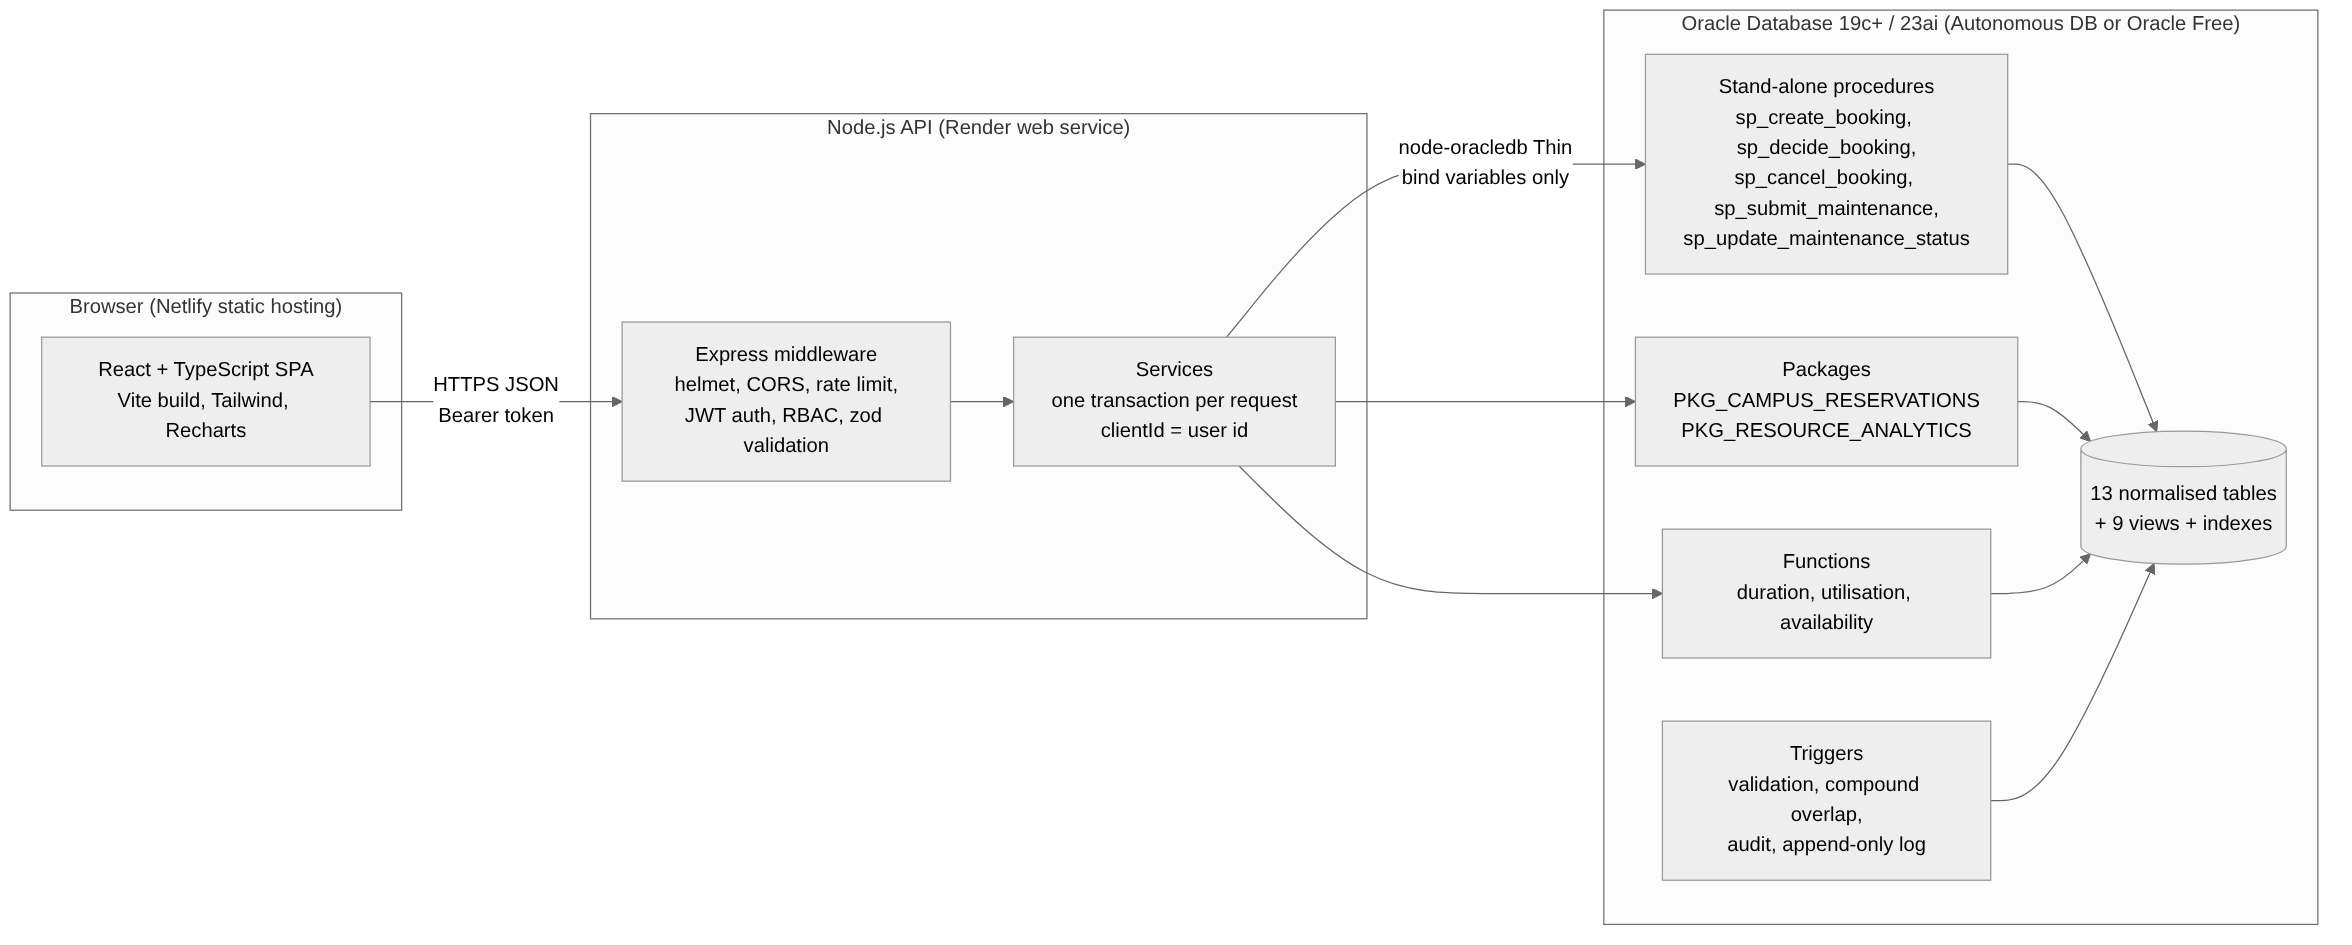
\includegraphics[width=\linewidth]{architecture.png}
\caption{System architecture: React front end, Express API and Oracle database objects}\label{fig:arch}
\end{figure}

\section{Entities, Attributes and Relationships}
Table~\ref{tab:entities} lists the thirteen relations and the reason each exists. The Entity--Relationship diagram in Figure~\ref{fig:er} shows attributes, keys and cardinalities.

\begin{table}[H]\centering\small
\caption{Relations and their purpose}\label{tab:entities}
\begin{tabularx}{\linewidth}{@{}lX@{}}\toprule
Relation & Purpose\\\midrule
ROLES & authorisation level; flags \texttt{can\_approve}, \texttt{can\_administer}\\
DEPARTMENTS & schools and offices that own users and resources\\
USERS & everyone who can sign in (bcrypt password hash, unique e-mail)\\
BUILDINGS & physical buildings\\
RESOURCE\_CATEGORIES & booking policy shared by a class of resources (approval, maximum hours, notice)\\
RESOURCES & anything bookable: status, capacity, operating hours, JSON features\\
BOOKINGS & one reservation of one resource for one half-open interval $[s,e)$\\
BOOKING\_APPROVALS & the single decision on a booking (one-to-one with BOOKINGS)\\
MAINTENANCE\_REQUESTS & fault tickets; \texttt{blocks\_booking} takes a resource out of service\\
RESOURCE\_BLACKOUTS & scheduled unavailability (exams, holidays, servicing)\\
AUDIT\_LOGS & append-only change history written only by triggers\\
NOTIFICATIONS & in-application messages\\
UTILISATION\_SNAPSHOTS & dated output of the utilisation reporting cursor\\\bottomrule
\end{tabularx}\end{table}

\begin{figure}[H]\centering
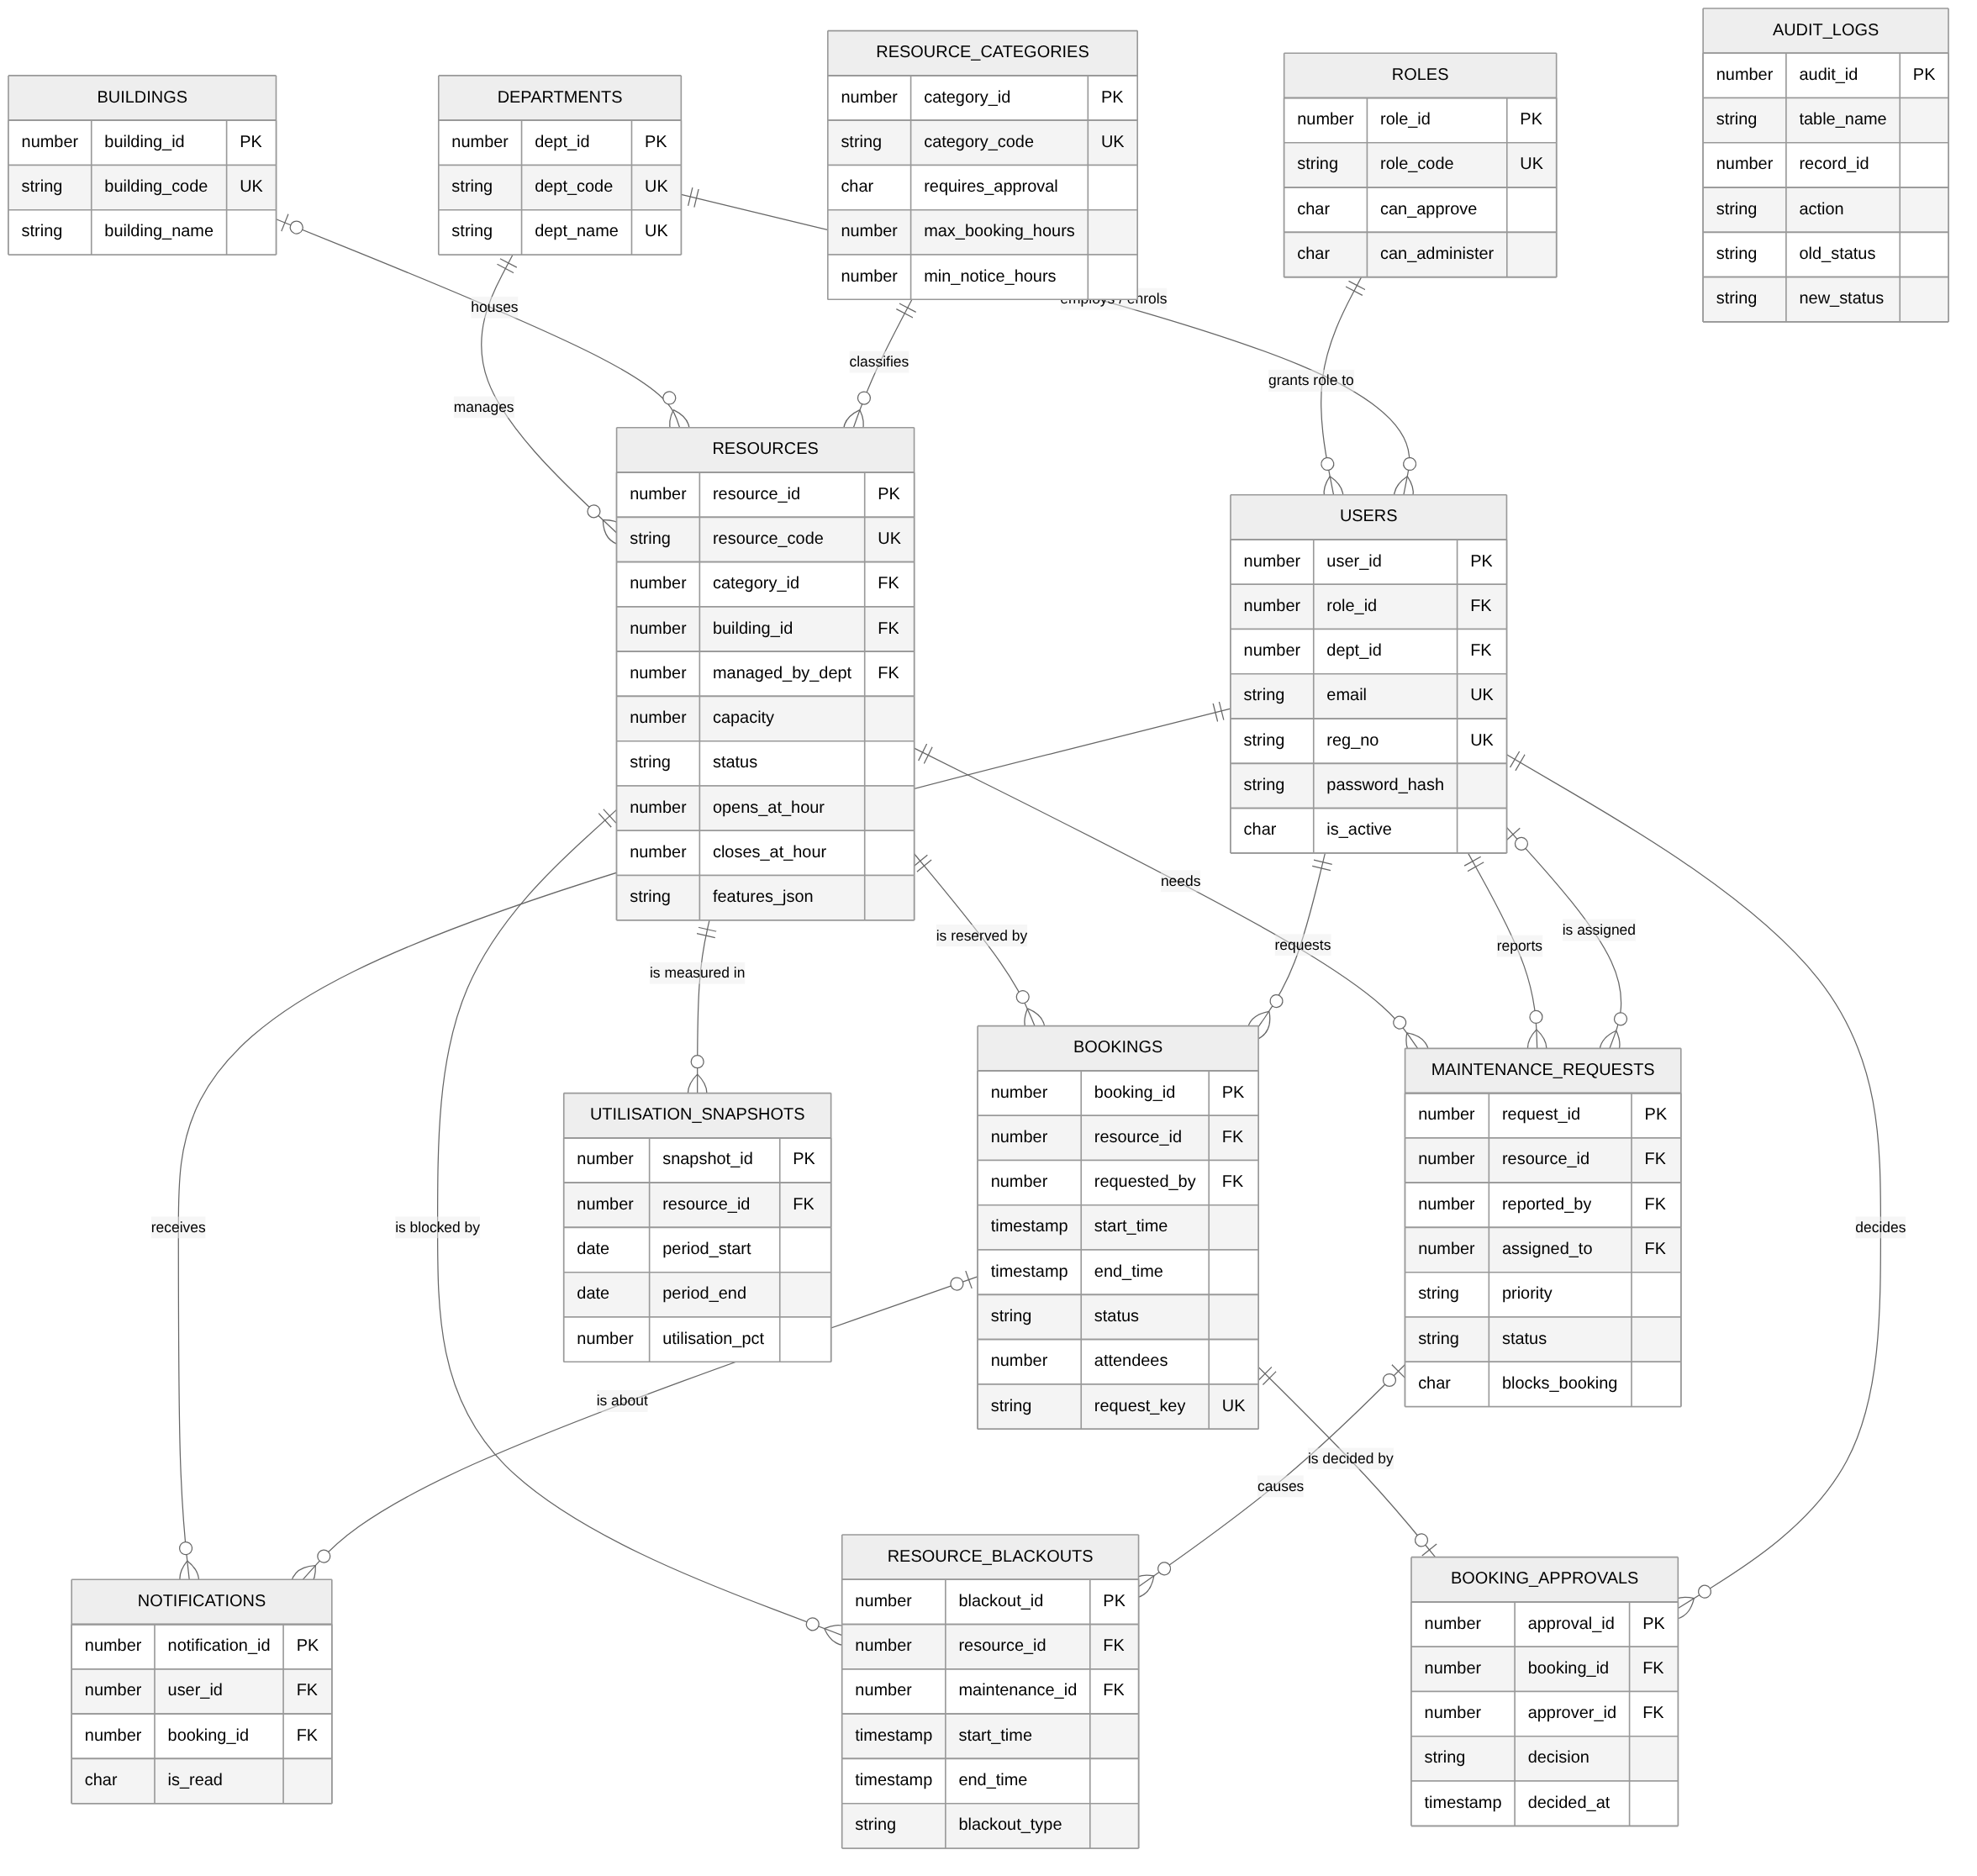
\includegraphics[width=\linewidth,height=0.62\textheight,keepaspectratio]{er_diagram.png}
\caption{Entity--Relationship diagram of CampusReserve (crow's-foot notation)}\label{fig:er}
\end{figure}

Key relationship decisions:
\begin{itemize}
  \item \textbf{BUILDINGS 0..1 to many RESOURCES.} Portable equipment has no building, so \texttt{building\_id} is nullable.
  \item \textbf{BOOKINGS 1 to 0..1 BOOKING\_APPROVALS.} A unique constraint on \texttt{booking\_id} guarantees at most one decision; re-deciding is impossible at the data level.
  \item \textbf{USERS to MAINTENANCE\_REQUESTS} appears twice, as reporter (mandatory) and assignee (optional).
  \item \textbf{AUDIT\_LOGS has no foreign key.} Audit rows must outlive the rows they describe and must never block a delete; they reference records through \texttt{(table\_name, record\_id)}.
\end{itemize}

\section{Mapping the ER Model to Relations}
Each strong entity became a table with a surrogate identity primary key; natural codes (e-mail, resource code, department code) are kept as \texttt{UNIQUE} candidate keys. Each one-to-many relationship became a foreign key on the ``many'' side. The one-to-one decision relationship became a foreign key with a unique constraint. Multi-valued descriptive features of a resource (projector, GPU count) are stored in a validated JSON column because they are never joined or aggregated. Figure~\ref{fig:schema} shows the resulting relational schema.

\begin{figure}[H]\centering
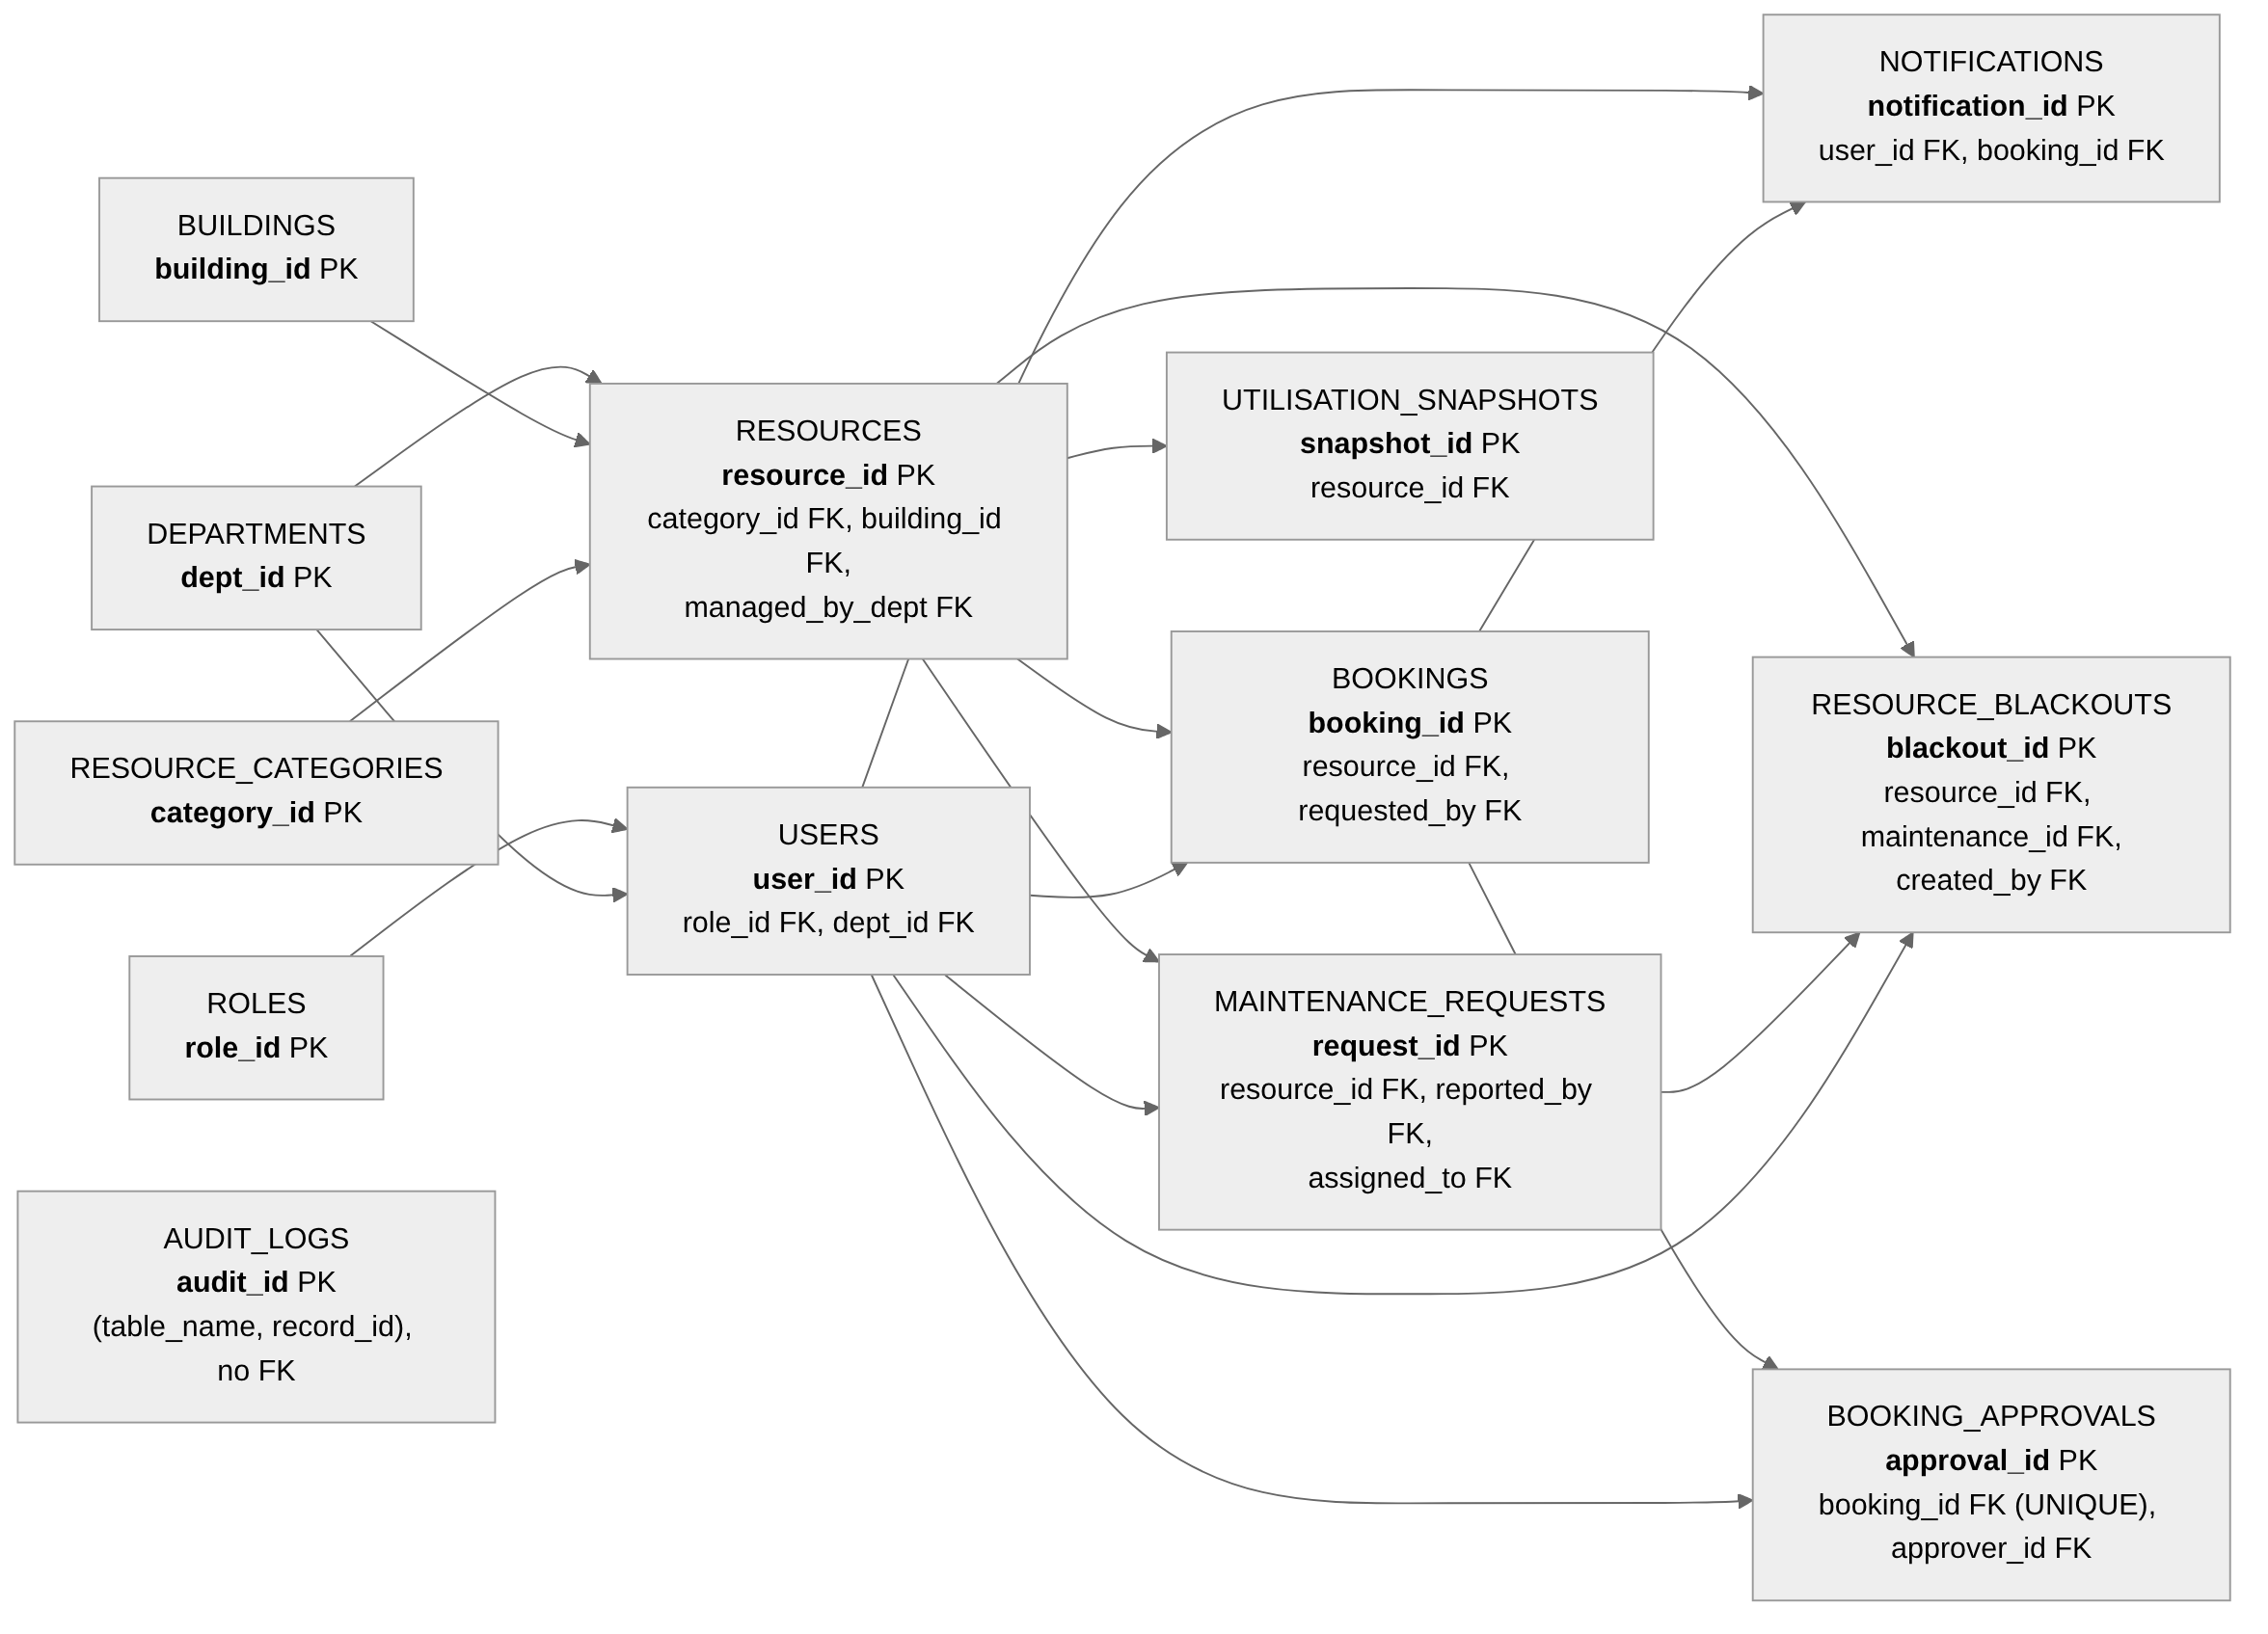
\includegraphics[width=\linewidth,height=0.5\textheight,keepaspectratio]{relational_schema.png}
\caption{Relational schema: primary keys and foreign-key references between the thirteen tables}\label{fig:schema}
\end{figure}

\section{Schema Definitions with Constraints}
Tables are created in \texttt{01\_create\_schema.sql} with primary keys, \texttt{NOT NULL} and \texttt{DEFAULT}; all other constraints are added with \texttt{ALTER TABLE} in \texttt{02\_constraints\_indexes.sql}, which exercises the full DDL syllabus (\texttt{CREATE}, \texttt{ALTER}, \texttt{DROP}). Listing~\ref{lst:ddl} shows the central BOOKINGS table.

\begin{lstlisting}[language=PLSQL,caption={BOOKINGS table and its constraints (excerpt)},label=lst:ddl]
CREATE TABLE bookings (
    booking_id     NUMBER(12)     GENERATED BY DEFAULT AS IDENTITY,
    resource_id    NUMBER(10)     NOT NULL,
    requested_by   NUMBER(10)     NOT NULL,
    title          VARCHAR2(150)  NOT NULL,
    attendees      NUMBER(5)      DEFAULT 1 NOT NULL,
    start_time     TIMESTAMP      NOT NULL,
    end_time       TIMESTAMP      NOT NULL,
    status         VARCHAR2(12)   DEFAULT 'PENDING' NOT NULL,
    request_key    VARCHAR2(64),               -- idempotency key
    cancelled_at   TIMESTAMP,
    ...
    CONSTRAINT pk_bookings PRIMARY KEY (booking_id));

ALTER TABLE bookings ADD CONSTRAINT ck_bookings_interval CHECK (end_time > start_time);
ALTER TABLE bookings ADD CONSTRAINT ck_bookings_status
    CHECK (status IN ('PENDING','APPROVED','REJECTED','CANCELLED'));
ALTER TABLE bookings ADD CONSTRAINT ck_bookings_cancel
    CHECK ((status = 'CANCELLED' AND cancelled_at IS NOT NULL)
        OR (status <> 'CANCELLED' AND cancelled_at IS NULL));
ALTER TABLE bookings ADD CONSTRAINT uq_bookings_request_key UNIQUE (request_key);
ALTER TABLE bookings ADD CONSTRAINT fk_bookings_resource
    FOREIGN KEY (resource_id) REFERENCES resources (resource_id);
\end{lstlisting}

\begin{table}[H]\centering\small
\caption{Constraint inventory}\label{tab:constraints}
\begin{tabularx}{\linewidth}{@{}lp{1.2cm}X@{}}\toprule
Type & Count & Examples and purpose\\\midrule
PRIMARY KEY & 13 & one per table; identity columns except the fixed role IDs\\
FOREIGN KEY & 18 & named \texttt{fk\_*}; \texttt{ON DELETE CASCADE} only for dependent data (approvals, notifications, snapshots), \texttt{ON DELETE SET NULL} for optional links\\
UNIQUE & 11 & e-mail, registration number, codes, request key, one decision per booking, one snapshot per resource and period\\
CHECK & 29 & interval order, status domains, cancelled $\Leftrightarrow$ \texttt{cancelled\_at}, resolved $\Leftrightarrow$ \texttt{resolved\_at}, operating hours, capacity $\ge 0$, e-mail pattern (\texttt{REGEXP\_LIKE}), \texttt{features\_json IS JSON}\\
NOT NULL / DEFAULT & -- & every mandatory column; defaults for statuses, flags and timestamps\\\bottomrule
\end{tabularx}\end{table}

Rules that depend on \emph{other rows} --- overlap, approval rights, maintenance state --- cannot be expressed as \texttt{CHECK} constraints in Oracle. They are enforced by stored procedures and triggers (Chapter~\ref{ch:impl}).

\section{Normalisation}
Figure~\ref{fig:norm} summarises the decomposition from an unnormalised booking register to the final schema.

\begin{figure}[H]\centering
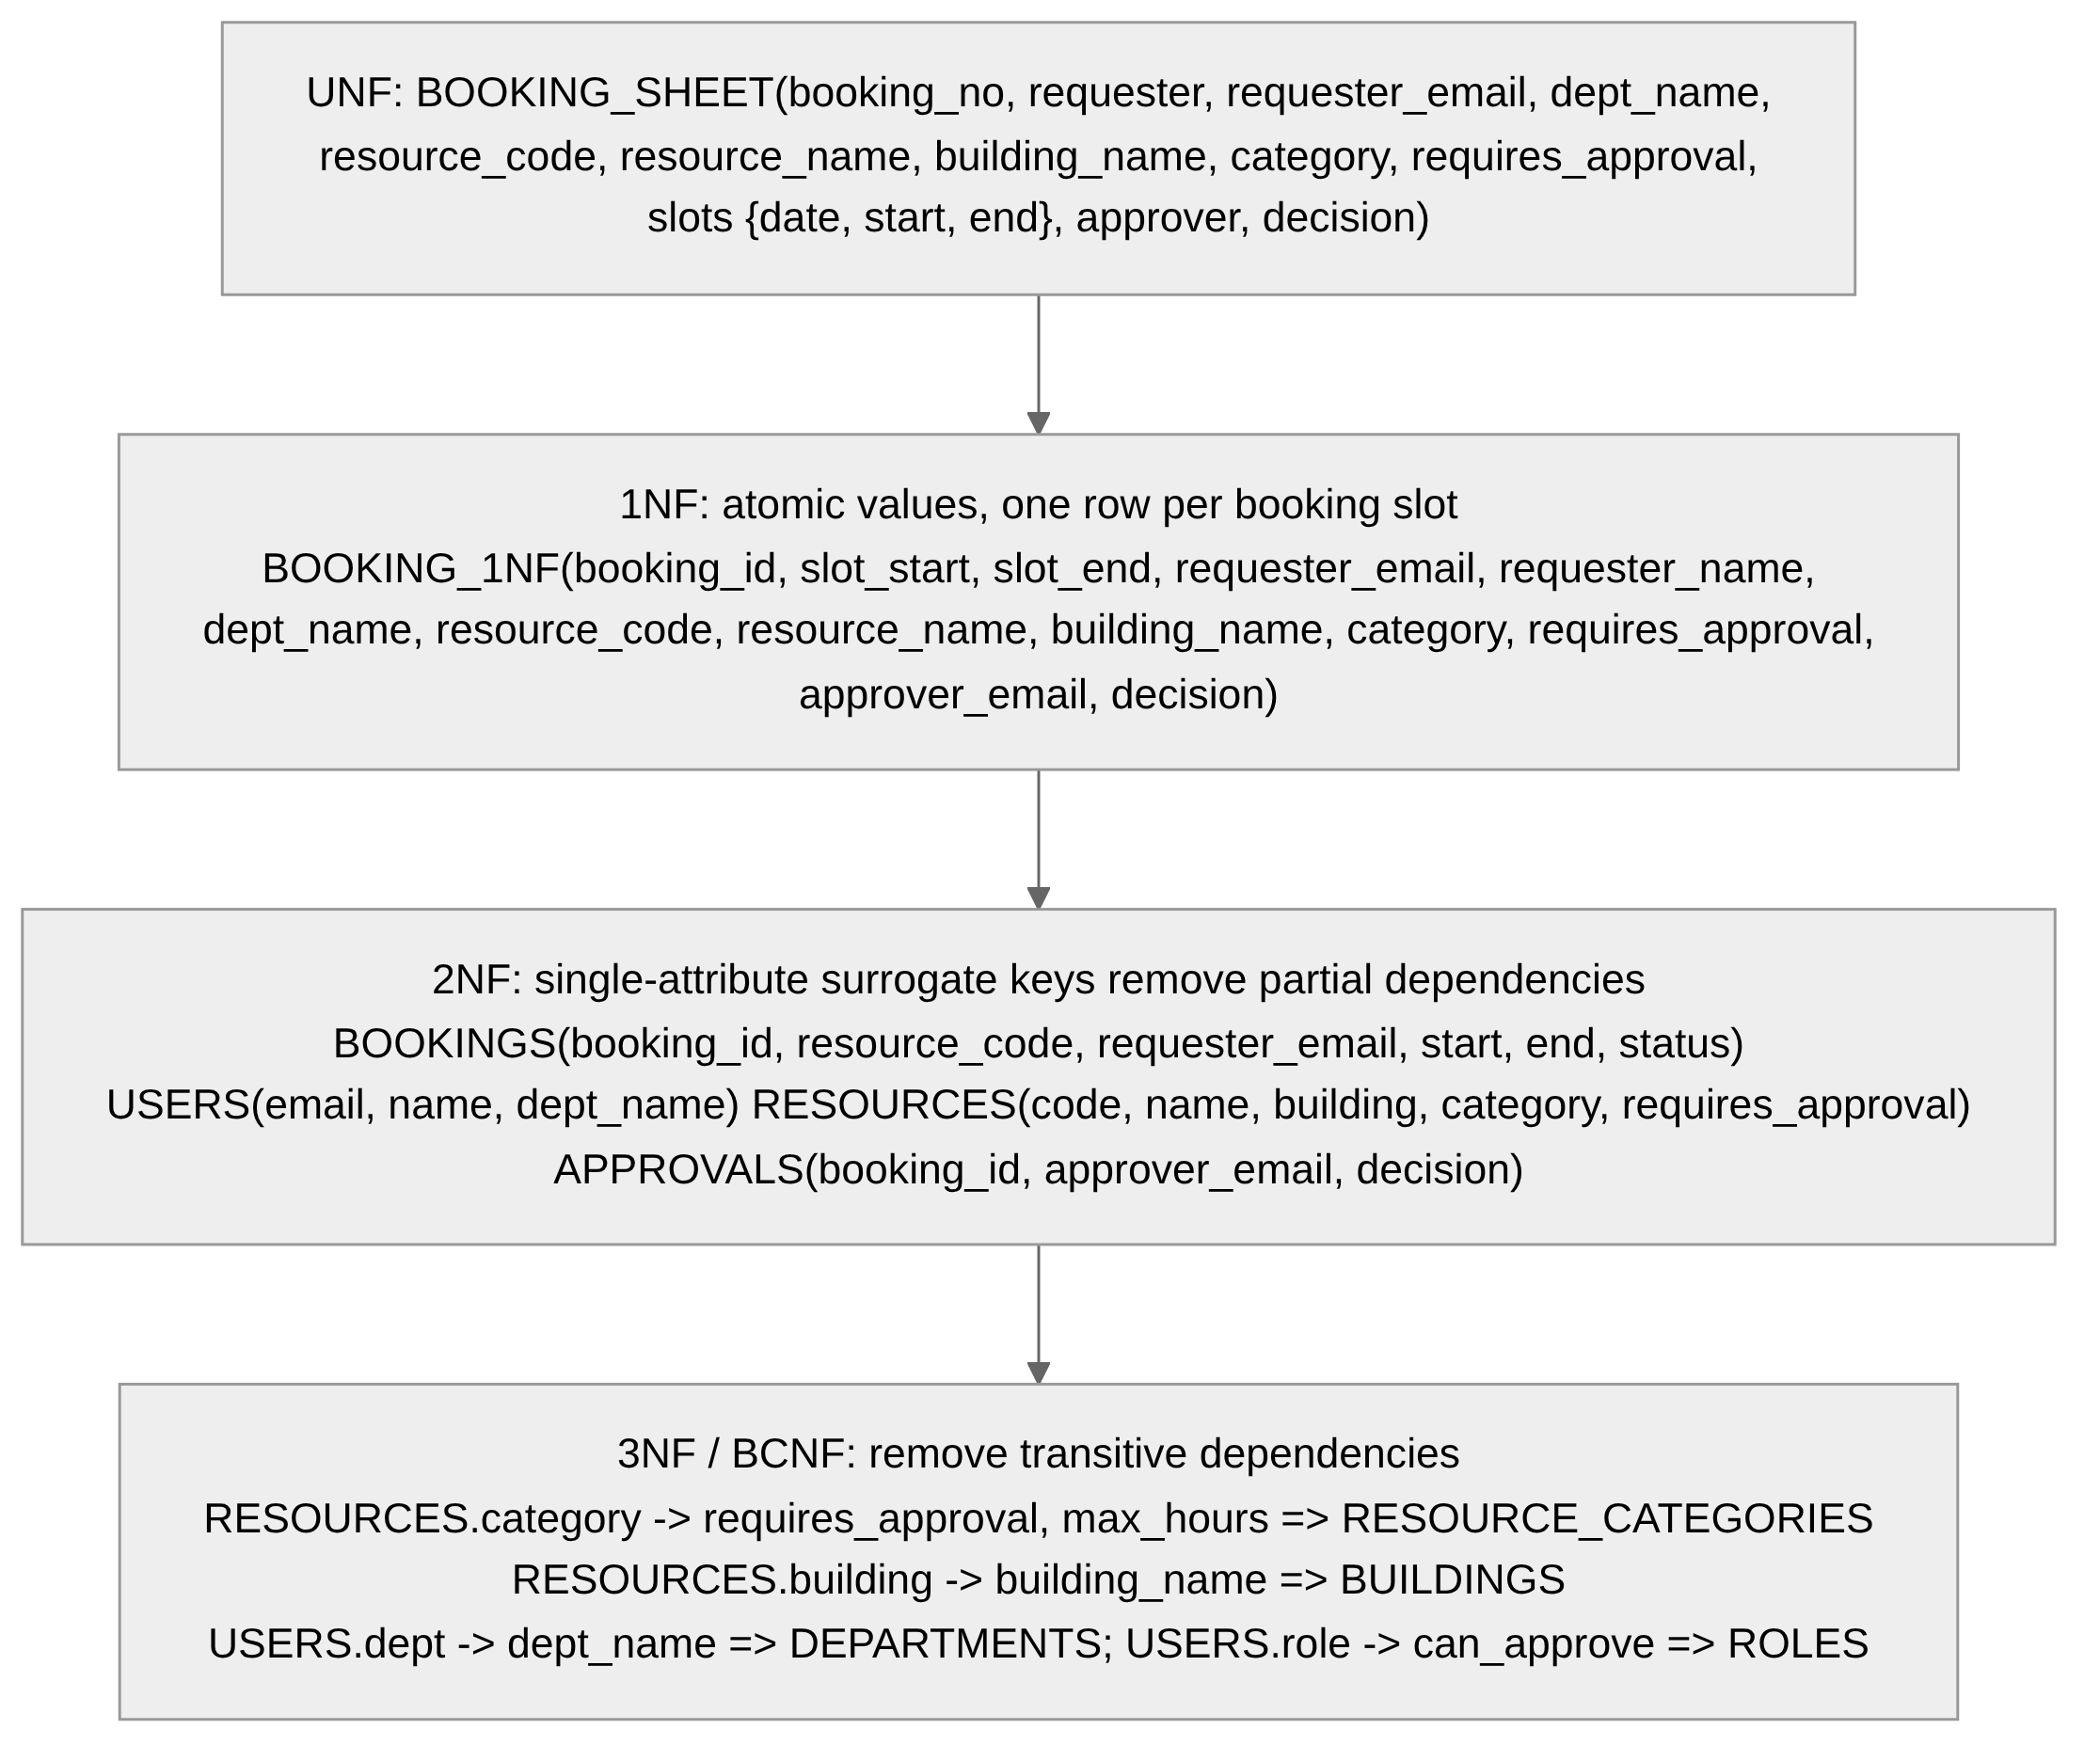
\includegraphics[width=0.92\linewidth,height=0.42\textheight,keepaspectratio]{normalisation.png}
\caption{Normalisation steps from the unnormalised booking register to 3NF/BCNF}\label{fig:norm}
\end{figure}

\subsection{Unnormalised form}
A typical paper or spreadsheet register records, per request, the requester's name, e-mail and department, the resource code, name, building and category, the category's approval rule, a \emph{list} of requested dates and times, and the approver's details and decision:

\texttt{BOOKING\_SHEET(booking\_no, requester\_name, requester\_email, requester\_dept, resource\_code, resource\_name, building\_name, category, requires\_approval, max\_hours, \{date, start, end\}, approver\_email, approver\_name, decision)}

The braces mark a repeating group.

\subsection{First normal form}
The repeating group is removed so that every attribute is atomic and each row describes exactly one interval; each interval becomes its own booking with key \texttt{booking\_id}:

\texttt{BOOKING\_1NF(booking\_id, start\_time, end\_time, requester\_email, requester\_name, requester\_dept, dept\_name, resource\_code, resource\_name, building\_code, building\_name, category, requires\_approval, max\_hours, approver\_email, approver\_name, decision)}

\subsection{Functional dependencies}
\begin{table}[H]\centering\small
\caption{Functional dependencies identified in BOOKING\_1NF}\label{tab:fd}
\begin{tabularx}{\linewidth}{@{}lX@{}}\toprule
Determinant & Dependent attributes\\\midrule
booking\_id & start\_time, end\_time, requester\_email, resource\_code, status, approver\_email, decision\\
requester\_email & requester\_name, requester\_dept, role\\
requester\_dept & dept\_name\\
role & can\_approve, can\_administer\\
resource\_code & resource\_name, building\_code, category, capacity, operating hours, managing department\\
building\_code & building\_name, campus\_zone\\
category & requires\_approval, max\_hours, min\_notice\_hours\\
approver\_email & approver\_name\\\bottomrule
\end{tabularx}\end{table}

\subsection{Second normal form}
With the single-attribute key \texttt{booking\_id} there is no partial dependency, so BOOKING\_1NF is formally in 2NF. Had the natural composite key \texttt{(resource\_code, start\_time)} been used, \texttt{resource\_name}, \texttt{building\_code} and \texttt{category} would depend on only part of it --- a partial dependency. In both cases the entity data is separated into \texttt{BOOKINGS}, \texttt{USERS}, \texttt{RESOURCES} and \texttt{APPROVALS}, each with facts about one thing only.

\subsection{Third normal form}
Transitive dependencies (non-key determining non-key) remain in the 2NF relations and are removed by decomposition:
\begin{itemize}
  \item resource\_code $\rightarrow$ category $\rightarrow$ requires\_approval, max\_hours \quad gives RESOURCE\_CATEGORIES;
  \item resource\_code $\rightarrow$ building\_code $\rightarrow$ building\_name \quad gives BUILDINGS;
  \item email $\rightarrow$ dept $\rightarrow$ dept\_name \quad gives DEPARTMENTS;
  \item email $\rightarrow$ role $\rightarrow$ can\_approve \quad gives ROLES.
\end{itemize}
Without this step, changing a category's approval rule would require updating every resource row (update anomaly), and a category with no resources could not be recorded (insertion anomaly).

\subsection{Boyce--Codd normal form}
A relation is in BCNF when every non-trivial determinant is a candidate key. In the final schema the only determinants are the surrogate keys and the declared unique keys (\texttt{email}, \texttt{reg\_no}, \texttt{resource\_code}, the reference-table codes, \texttt{request\_key}, \texttt{booking\_id} in BOOKING\_APPROVALS and \texttt{(resource\_id, period\_start, period\_end)} in UTILISATION\_SNAPSHOTS), all of which are candidate keys. The pair \texttt{(resource\_id, start\_time)} is deliberately \emph{not} unique: a cancelled or rejected booking may share a slot with a later live booking, so uniqueness of live slots is an overlap rule rather than a functional dependency. Every relation is therefore in BCNF. Derived values --- duration and utilisation --- are not stored; they are computed by functions and views to avoid update anomalies.

\section{Indexes}
Oracle does not create indexes for foreign keys automatically. An unindexed foreign key causes full scans on joins and can lead to table-level locks on the child table when the parent key is modified. Twenty-two explicit indexes cover every foreign key (checked by query V5 in \texttt{13\_verification.sql}) and the three most frequent access paths:

\begin{table}[H]\centering\small
\caption{Access-path indexes}\label{tab:indexes}
\begin{tabularx}{\linewidth}{@{}lX@{}}\toprule
Index & Query it serves\\\midrule
ix\_bookings\_res\_time (resource\_id, start\_time, end\_time) & overlap check inside the booking procedure; calendar; utilisation\\
ix\_bookings\_user\_start (requested\_by, start\_time) & ``My bookings''\\
ix\_bookings\_status\_start (status, start\_time) & approval queue; dashboard counts\\
ix\_maint\_status\_priority, ix\_maint\_resource & maintenance board\\
ix\_audit\_record (table\_name, record\_id) & change history of one booking\\
ix\_notif\_user\_read (user\_id, is\_read, created\_at) & notification bell\\\bottomrule
\end{tabularx}\end{table}

% =============================================================================
% 8. IMPLEMENTATION
% =============================================================================
\chapter{Implementation}\label{ch:impl}

Table~\ref{tab:objects} lists every database object. The scripts are numbered in execution order and \texttt{run\_all.sql} installs them and stops if any object is invalid.

\begin{table}[H]\centering\small
\caption{Database objects implemented}\label{tab:objects}
\begin{tabularx}{\linewidth}{@{}lX@{}}\toprule
Type & Objects\\\midrule
Tables (13) & see Table~\ref{tab:entities}\\
Views (9) & v\_resource\_catalog, v\_booking\_details, v\_pending\_approvals, v\_active\_bookings, v\_maintenance\_dashboard, v\_resource\_utilisation\_30d, v\_department\_usage, v\_booking\_trend\_daily, v\_top\_resources\\
Functions (5) & fn\_booking\_duration\_hours, fn\_resource\_utilisation, fn\_resource\_availability; helpers fn\_hours\_between, fn\_current\_actor\\
Procedures (5) & sp\_create\_booking, sp\_decide\_booking, sp\_cancel\_booking, sp\_submit\_maintenance, sp\_update\_maintenance\_status\\
Packages (2) & pkg\_campus\_reservations, pkg\_resource\_analytics (specification and body)\\
Triggers (9) & trg\_users\_biu, trg\_resources\_bu, trg\_bookings\_biu, trg\_bookings\_no\_overlap (compound), trg\_bookings\_audit, trg\_maintenance\_biu, trg\_maintenance\_audit, trg\_resources\_status\_audit, trg\_audit\_logs\_immutable\\
Cursors & explicit (send\_pending\_digest), explicit \texttt{FOR UPDATE SKIP LOCKED} (expire\_stale\_pending), cursor \texttt{FOR} loops (escalate\_stale\_maintenance, sp\_submit\_maintenance, print\_utilisation\_report), parameterised cursor (build\_utilisation\_snapshot), REF cursors (seven package functions)\\\bottomrule
\end{tabularx}\end{table}

\section{SQL Coverage of the Syllabus}
The indicative experiments of the BCSE302P syllabus map to the implementation as shown in Table~\ref{tab:syllabus}.

\begin{table}[H]\centering\small
\caption{Syllabus experiments and where they are demonstrated}\label{tab:syllabus}
\begin{tabularx}{\linewidth}{@{}p{4.2cm}X@{}}\toprule
Syllabus experiment & Demonstration in CampusReserve\\\midrule
1. DDL and DML & \texttt{CREATE}/\texttt{ALTER}/\texttt{DROP} (01, 02, 00); \texttt{INSERT}, \texttt{UPDATE}, \texttt{DELETE} (seed, procedures, tests); \texttt{MERGE} (snapshot procedure)\\
2. Constraints & Table~\ref{tab:constraints}; violation tests TC-17 and TC-18\\
3. Single-row functions & \texttt{UPPER}, \texttt{LOWER}, \texttt{TRIM}, \texttt{NVL}, \texttt{NVL2}, \texttt{ROUND}, \texttt{TRUNC}, \texttt{LPAD}, \texttt{RPAD}, \texttt{SUBSTR}, \texttt{TO\_CHAR}, \texttt{EXTRACT}, \texttt{CAST}, \texttt{GREATEST}, \texttt{LEAST}, \texttt{NUMTODSINTERVAL}, \texttt{REGEXP\_LIKE}, \texttt{CASE}\\
4. Operators and group functions & \texttt{IN}, \texttt{BETWEEN}, \texttt{LIKE}, comparison and interval operators; \texttt{COUNT}, \texttt{SUM}, \texttt{AVG}, \texttt{MIN}, \texttt{MAX}, \texttt{COUNT(DISTINCT)}; \texttt{GROUP BY}/\texttt{HAVING} in v\_department\_usage; \texttt{DENSE\_RANK} and \texttt{COUNT(*) OVER()} analytic functions\\
5. Subqueries, views and joins & scalar and correlated subqueries (v\_resource\_catalog, v\_pending\_approvals), \texttt{NOT EXISTS} (verification V5), inner, left outer, cross and self joins (overlap self-join V7), \texttt{UNION ALL} (resource\_schedule), nine views\\
6. Procedures, functions, cursors, triggers & Sections~\ref{sec:fn}--\ref{sec:cur}\\\bottomrule
\end{tabularx}\end{table}

Listing~\ref{lst:view} shows a view that combines a left outer join, aggregates and \texttt{HAVING}.

\begin{lstlisting}[language=PLSQL,caption={Department usage view with GROUP BY and HAVING},label=lst:view]
CREATE OR REPLACE VIEW v_department_usage AS
SELECT d.dept_code, d.dept_name,
       COUNT(bk.booking_id)                                     AS total_requests,
       SUM(CASE WHEN bk.status = 'APPROVED' THEN 1 ELSE 0 END)  AS approved,
       ROUND(SUM(CASE WHEN bk.status = 'APPROVED'
                      THEN (CAST(bk.end_time AS DATE) - CAST(bk.start_time AS DATE)) * 24
                      ELSE 0 END), 1)                           AS approved_hours,
       COUNT(DISTINCT bk.resource_id)                           AS distinct_resources
FROM departments d
JOIN users u     ON u.dept_id = d.dept_id
JOIN bookings bk ON bk.requested_by = u.user_id
GROUP BY d.dept_id, d.dept_code, d.dept_name
HAVING COUNT(bk.booking_id) > 0;
\end{lstlisting}

\section{Functions}\label{sec:fn}
Functions have no side effects so they can be called from SQL as well as PL/SQL.

\begin{table}[H]\centering\small
\caption{Functions: parameters and results}\label{tab:fn}
\begin{tabularx}{\linewidth}{@{}lXX@{}}\toprule
Function & Input & Output\\\midrule
fn\_booking\_duration\_hours & p\_booking\_id & hours (2 dp); ORA-20010 if missing\\
fn\_resource\_utilisation & p\_resource\_id, p\_from (incl.), p\_to (excl.) & percentage of operating hours booked\\
fn\_resource\_availability & p\_resource\_id, p\_start, p\_end, p\_ignore\_booking & AVAILABLE, INVALID\_INTERVAL, NOT\_FOUND, MAINTENANCE, RETIRED, OUTSIDE\_HOURS, BLACKOUT or CONFLICT\\\bottomrule
\end{tabularx}\end{table}

\textbf{Utilisation logic.} Approved hours are summed only for bookings that intersect the window, and each booking is clipped to the window with \texttt{GREATEST}/\texttt{LEAST} so that a booking straddling the boundary is counted only for the part inside. The denominator is the number of days in the window multiplied by the resource's daily operating hours.

\begin{lstlisting}[language=PLSQL,caption={Utilisation function (core)},label=lst:util]
SELECT NVL(SUM(fn_hours_between(GREATEST(start_time, v_from_ts),
                                LEAST(end_time, v_to_ts))), 0)
  INTO v_booked
  FROM bookings
 WHERE resource_id = p_resource_id AND status = 'APPROVED'
   AND start_time < v_to_ts AND end_time > v_from_ts;
v_available := (TRUNC(p_to) - TRUNC(p_from)) * (v_close - v_open);
RETURN LEAST(100, ROUND(100 * v_booked / v_available, 2));
\end{lstlisting}

\textbf{Availability logic.} Two half-open intervals $[s_1,e_1)$ and $[s_2,e_2)$ overlap if and only if $s_1 < e_2 \wedge s_2 < e_1$~\cite{allen}. Using half-open intervals means a booking ending at 12:00 and another starting at 12:00 do not conflict, which test TC-06b checks. The function is \emph{advisory}: it powers the live ``This time is free'' indicator in the booking form, but the final decision is always made by \texttt{sp\_create\_booking} under a lock.

\textbf{Example.} \texttt{SELECT fn\_resource\_availability(1, TIMESTAMP '2026-11-20 10:00:00', TIMESTAMP '2026-11-20 12:00:00') FROM dual;} is expected to return \texttt{AVAILABLE} on an empty slot and \texttt{CONFLICT} after a booking is placed there. Actual output: Figure~\ref{fig:ev-fn}.

\evidence{fig08_functions.png}{Function outputs from verification script section V8 (own execution)\label{fig:ev-fn}}

\section{Stored Procedures and Transaction-safe Booking}\label{sec:proc}

\begin{table}[H]\centering\small
\caption{Stored procedures}\label{tab:proc}
\begin{tabularx}{\linewidth}{@{}lXX@{}}\toprule
Procedure & IN parameters & OUT / effect\\\midrule
sp\_create\_booking & resource, user, title, purpose, attendees, start, end, request key & o\_booking\_id, o\_status (PENDING/APPROVED), o\_duplicate\\
sp\_decide\_booking & booking, approver, decision, remarks & status change, approval row, notification\\
sp\_cancel\_booking & booking, user, reason & CANCELLED, slot freed, notification\\
sp\_submit\_maintenance & resource, user, title, description, priority, blocks\_booking & o\_request\_id; resource set to MAINTENANCE if blocking; holders notified\\
sp\_update\_maintenance\_status & request, actor, new status, assignee, notes & ticket updated; resource status recomputed\\\bottomrule
\end{tabularx}\end{table}

\subsection{Why a simple overlap check is not enough}
A naive implementation runs \texttt{SELECT COUNT(*)} for overlapping bookings and inserts when the count is zero. Under Oracle's default \texttt{READ COMMITTED} isolation each statement sees only data committed before it began. If sessions A and B both run the check before either commits, both see zero and both insert; the overlap is committed. This is the classic phantom problem described by Eswaran et al.~\cite{eswaran} and analysed for SQL isolation levels by Berenson et al.~\cite{berenson}: the conflicting row does not yet exist, so there is nothing for an ordinary row lock to protect.

\subsection{Concurrency-safe design}
\texttt{sp\_create\_booking} serialises all writers \emph{per resource} by locking the parent \texttt{RESOURCES} row before checking (Listing~\ref{lst:create}). The resource row acts as a lock object for the set of its bookings, standing in for the predicate lock that Oracle does not provide. The second session blocks at the \texttt{SELECT~...~FOR~UPDATE}; when the first commits, the second resumes, and its overlap query --- a \emph{new} statement --- sees the committed booking and raises ORA-20005 (Figure~\ref{fig:seq}). Requests for \emph{different} resources never wait for each other. \texttt{WAIT 5} turns an unusually long wait into ORA-20018 (``resource busy, retry'') instead of hanging the API.

\begin{lstlisting}[language=PLSQL,caption={sp\_create\_booking: serialisation point and overlap check (excerpt)},label=lst:create]
-- (d) SERIALISATION POINT: lock the resource row.
SELECT r.status, r.capacity, r.opens_at_hour, r.closes_at_hour, ...
  INTO v_res_status, v_capacity, v_open, v_close, ...
  FROM resources r
  JOIN resource_categories c ON c.category_id = r.category_id
 WHERE r.resource_id = p_resource_id
   FOR UPDATE OF r.status WAIT 5;
-- (e) resource rules: maintenance, capacity, hours, max duration, notice, blackout
IF v_res_status = 'MAINTENANCE' THEN
    RAISE_APPLICATION_ERROR(-20003, v_res_name || ' is under maintenance ...');
END IF;
...
-- (f) overlap check, made while holding the lock
SELECT MIN(booking_id) INTO v_conflict_id
  FROM bookings
 WHERE resource_id = p_resource_id
   AND status IN ('PENDING', 'APPROVED')
   AND start_time < p_end AND end_time > p_start;
IF v_conflict_id IS NOT NULL THEN
    RAISE_APPLICATION_ERROR(-20005, 'Time slot conflicts with booking #' || v_conflict_id || '.');
END IF;
-- (g) accept: no COMMIT here - the caller owns the transaction
INSERT INTO bookings (...) VALUES (...) RETURNING booking_id INTO o_booking_id;
\end{lstlisting}

\begin{figure}[H]\centering
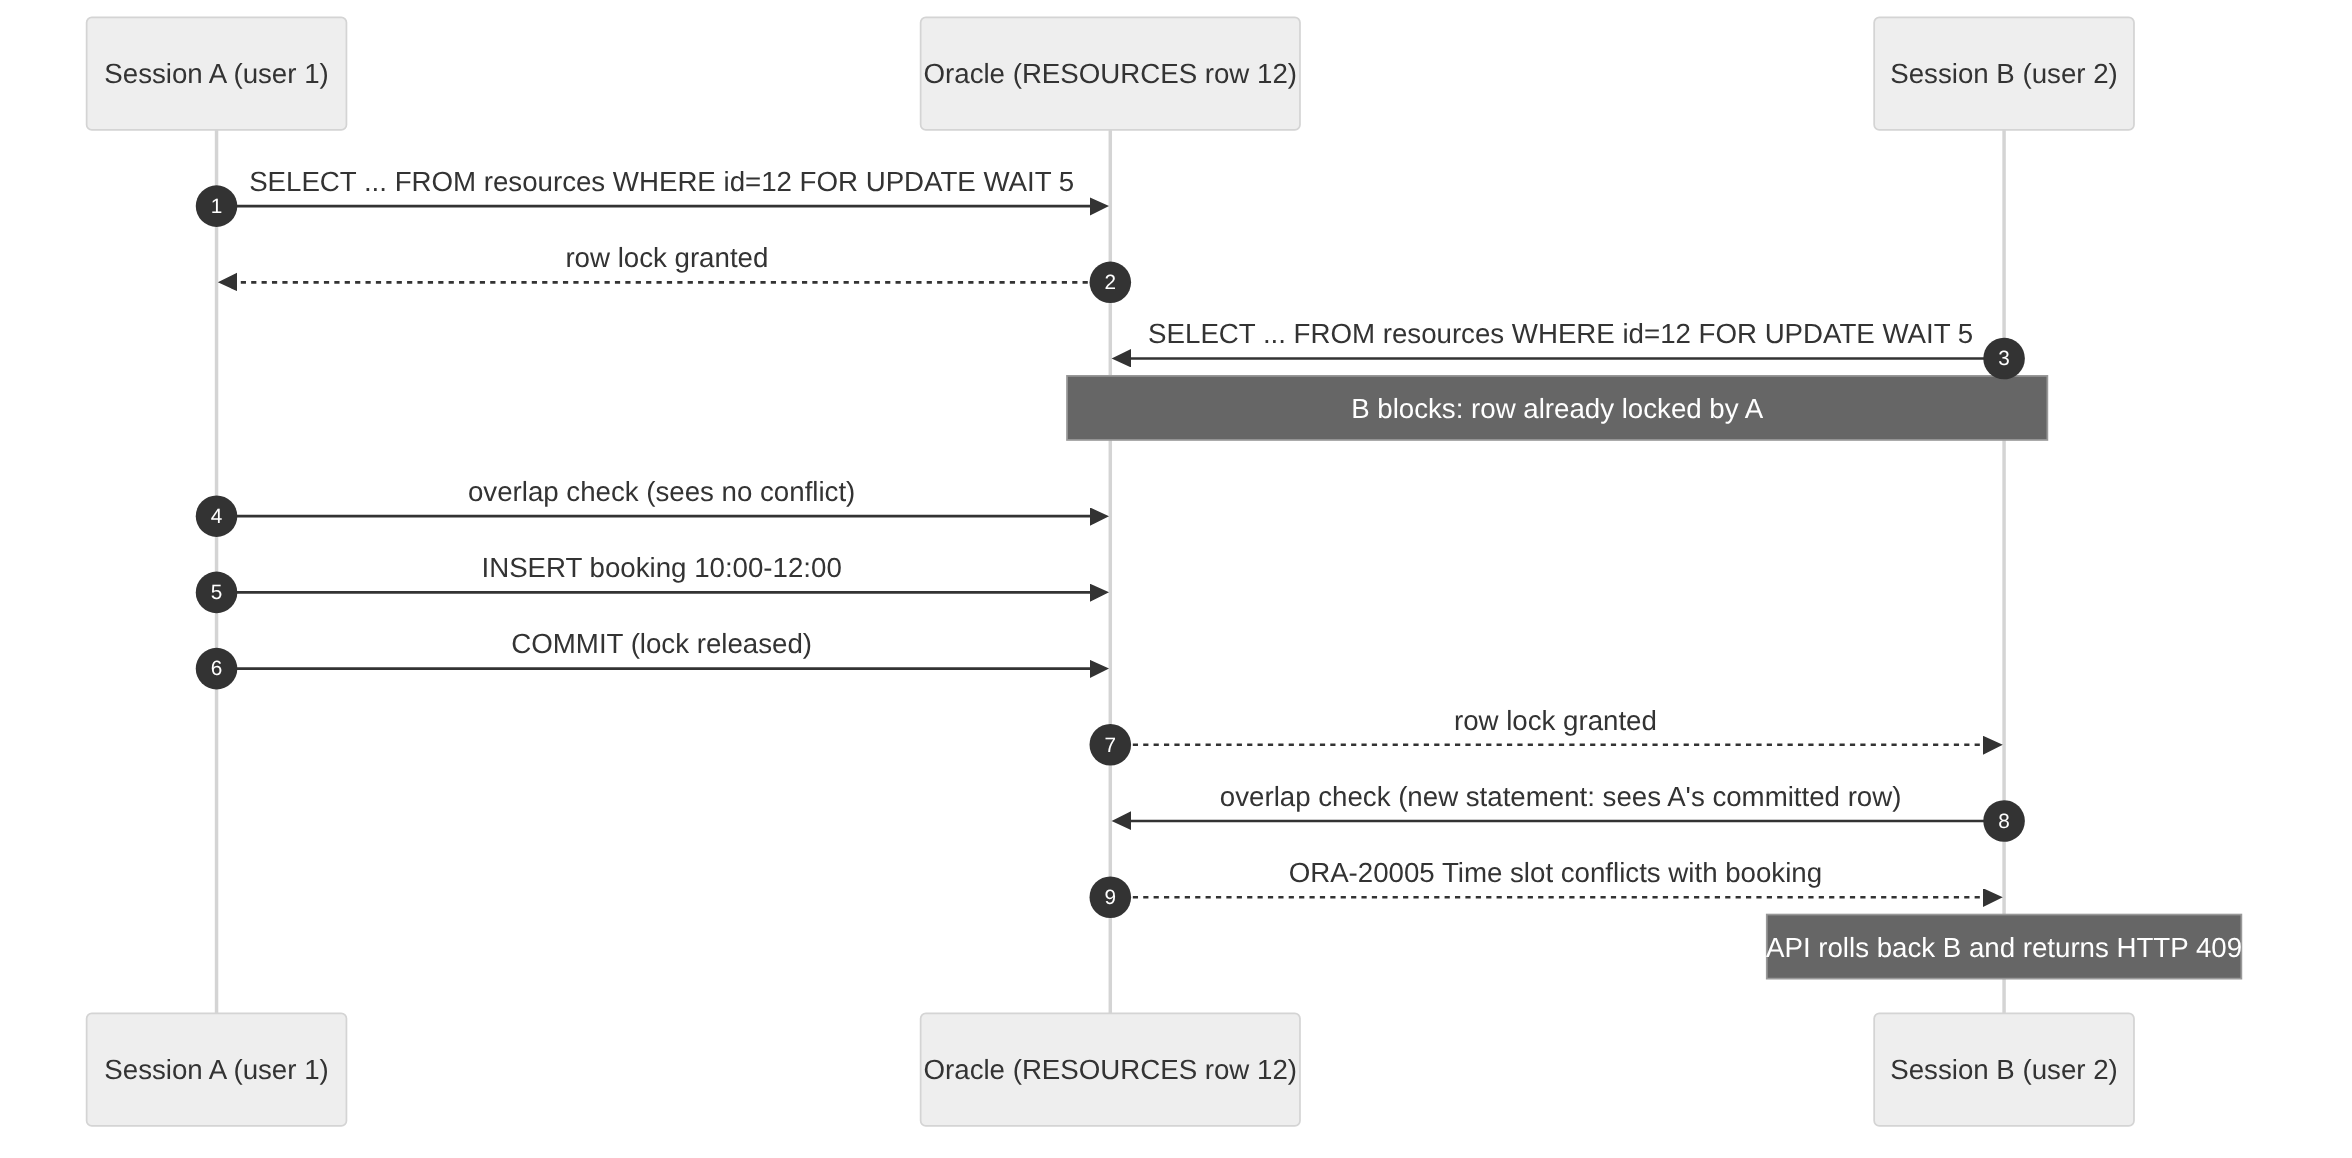
\includegraphics[width=0.86\linewidth]{concurrency_sequence.png}
\caption{Two sessions competing for the same slot: the row lock serialises them}\label{fig:seq}
\end{figure}

Further safeguards:
\begin{itemize}
  \item \textbf{Lock ordering.} Every procedure locks RESOURCES before BOOKINGS or MAINTENANCE\_REQUESTS, which removes the circular wait needed for a deadlock.
  \item \textbf{No commits in procedures.} The procedures never \texttt{COMMIT} or \texttt{ROLLBACK}. The API wraps each request in one transaction (Listing~\ref{lst:tx}), so a multi-step operation is atomic and the SQL test scripts can roll back everything they do.
  \item \textbf{Idempotency.} The client sends a random \texttt{Idempotency-Key}; a retried request returns the original booking instead of creating a duplicate (TC-18g). A race between two retries is caught by the unique constraint (\texttt{DUP\_VAL\_ON\_INDEX}).
  \item \textbf{Authorisation in the database.} \texttt{sp\_decide\_booking} checks that the approver's role can approve and, for coordinators, that the resource belongs to their department.
\end{itemize}

\begin{lstlisting}[language=Java,caption={API transaction wrapper (backend/src/config/db.js, excerpt)},label=lst:tx]
export async function withTransaction(actorId, fn) {
  const conn = await pool.getConnection();
  conn.clientId = actorId ? String(actorId) : '';   // read by audit triggers
  try {
    const result = await fn(conn);                  // e.g. BEGIN sp_create_booking(...); END;
    await conn.commit();                            // one commit per API request
    return result;
  } catch (err) {
    await conn.rollback();                          // any failure undoes the whole unit
    throw err;
  } finally {
    await conn.close();
  }
}
\end{lstlisting}

\textbf{Execution example (SQL*Plus).}
\begin{lstlisting}[language=PLSQL,caption={Calling sp\_create\_booking}]
VARIABLE id NUMBER
VARIABLE st VARCHAR2(12)
VARIABLE dup NUMBER
EXEC sp_create_booking(1, 7, 'DBMS project review', NULL, 12, -
     TIMESTAMP '2026-11-20 10:00:00', TIMESTAMP '2026-11-20 12:00:00', NULL, :id, :st, :dup);
PRINT id st
\end{lstlisting}
Expected output: a new booking ID and status \texttt{PENDING} (computer laboratories require approval). Repeating the call returns ORA-20005. Actual output is part of the test-suite evidence in Chapter~\ref{ch:test}.

\section{Packages}\label{sec:pkg}
Each package has a separate specification (\texttt{07\_package\_specifications.sql}) and body (\texttt{08\_package\_bodies.sql}).

\textbf{PKG\_CAMPUS\_RESERVATIONS} holds the reservation workflow helpers: status constants; named exceptions bound to the application error codes with \texttt{PRAGMA EXCEPTION\_INIT} (so PL/SQL callers can write \texttt{WHEN pkg\_campus\_reservations.e\_booking\_conflict}); the pipelined function \texttt{day\_slots} that generates the hourly availability strip; the REF-cursor functions \texttt{resource\_schedule} (calendar, using \texttt{UNION ALL} of bookings and blackouts) and \texttt{pending\_for\_approver}; and the cursor procedures \texttt{send\_pending\_digest} and \texttt{expire\_stale\_pending}.

\textbf{PKG\_RESOURCE\_ANALYTICS} computes everything shown on the analytics page: \texttt{dashboard\_summary}, \texttt{booking\_trend} (with a \texttt{CONNECT BY} row generator so days with no bookings still appear), \texttt{top\_resources}, \texttt{department\_usage}, \texttt{resource\_utilisation}, \texttt{peak\_hours}, plus \texttt{build\_utilisation\_snapshot}, \texttt{escalate\_stale\_maintenance} and \texttt{print\_utilisation\_report}.

\begin{lstlisting}[language=PLSQL,caption={Package specification (excerpt)},label=lst:pkgspec]
CREATE OR REPLACE PACKAGE pkg_campus_reservations AS
    c_pending  CONSTANT VARCHAR2(12) := 'PENDING';
    e_booking_conflict EXCEPTION; PRAGMA EXCEPTION_INIT(e_booking_conflict, -20005);
    TYPE t_slot IS RECORD (slot_start TIMESTAMP, slot_end TIMESTAMP,
                           slot_state VARCHAR2(12), booking_id NUMBER);
    TYPE t_slot_tab IS TABLE OF t_slot;
    FUNCTION day_slots (p_resource_id IN NUMBER, p_day IN DATE,
                        p_slot_minutes IN NUMBER DEFAULT 60) RETURN t_slot_tab PIPELINED;
    FUNCTION resource_schedule (p_resource_id IN NUMBER, p_from IN TIMESTAMP,
                                p_to IN TIMESTAMP) RETURN SYS_REFCURSOR;
    FUNCTION pending_for_approver (p_approver_id IN NUMBER) RETURN SYS_REFCURSOR;
    PROCEDURE send_pending_digest  (p_approver_id IN NUMBER, o_pending_count OUT NUMBER);
    PROCEDURE expire_stale_pending (p_actor_id IN NUMBER, o_expired OUT NUMBER);
END pkg_campus_reservations;
\end{lstlisting}

\textbf{Execution example.} \texttt{SELECT * FROM TABLE(pkg\_campus\_reservations.day\_slots(12, TRUNC(SYSDATE)+1, 60));} returns one row per hour with state FREE, BOOKED, PENDING, BLACKOUT, PAST or CLOSED; for a resource open 08:00--20:00 it returns 12 rows (TC-22).

\evidence{fig08_refcursor.png}{REF cursor output of pkg\_resource\_analytics.dashboard\_summary and pipelined day\_slots (own execution)}

\section{Triggers}\label{sec:trg}

\begin{table}[H]\centering\small
\caption{Triggers}\label{tab:trg}
\begin{tabularx}{\linewidth}{@{}lp{3.2cm}X@{}}\toprule
Trigger & Timing & Purpose\\\midrule
trg\_bookings\_biu & before insert/update, row & new rows must be PENDING/APPROVED on an AVAILABLE resource within capacity; status state machine; sets \texttt{cancelled\_at}; blocks rescheduling of final bookings\\
trg\_bookings\_no\_overlap & compound & defence-in-depth overlap detection (below)\\
trg\_bookings\_audit & after insert/update/delete, row & audit row with old/new status and details\\
trg\_maintenance\_biu & before insert/update, row & ticket state machine; maintains \texttt{resolved\_at}\\
trg\_maintenance\_audit & after insert/update, row & audit of status, priority and assignment\\
trg\_resources\_status\_audit & after update of status, row, \texttt{WHEN} & audit of availability changes\\
trg\_resources\_bu, trg\_users\_biu & before, row & \texttt{updated\_at}; lower-case e-mail\\
trg\_audit\_logs\_immutable & before update/delete, statement & makes AUDIT\_LOGS append-only\\\bottomrule
\end{tabularx}\end{table}

\textbf{Avoiding mutating-table errors.} A row-level trigger on BOOKINGS may not query BOOKINGS (ORA-04091). The overlap trigger is therefore a \emph{compound} trigger: the row section only remembers the affected IDs, and the check runs in the \texttt{AFTER STATEMENT} section, when the table is no longer mutating (Listing~\ref{lst:compound}). Row-level triggers only read \emph{other} tables, which is permitted.

\begin{lstlisting}[language=PLSQL,caption={Compound overlap trigger},label=lst:compound]
CREATE OR REPLACE TRIGGER trg_bookings_no_overlap
FOR INSERT OR UPDATE OF start_time, end_time, status, resource_id ON bookings
COMPOUND TRIGGER
    TYPE t_ids IS TABLE OF bookings.booking_id%TYPE;
    g_ids t_ids := t_ids();
    AFTER EACH ROW IS
    BEGIN
        IF :NEW.status IN ('PENDING', 'APPROVED') THEN
            g_ids.EXTEND; g_ids(g_ids.LAST) := :NEW.booking_id;
        END IF;
    END AFTER EACH ROW;
    AFTER STATEMENT IS
        v_conflict bookings.booking_id%TYPE;
    BEGIN
        FOR i IN 1 .. g_ids.COUNT LOOP
            SELECT MIN(o.booking_id) INTO v_conflict
              FROM bookings b JOIN bookings o
                ON o.resource_id = b.resource_id AND o.booking_id <> b.booking_id
               AND o.status IN ('PENDING','APPROVED')
               AND o.start_time < b.end_time AND o.end_time > b.start_time
             WHERE b.booking_id = g_ids(i);
            IF v_conflict IS NOT NULL THEN
                RAISE_APPLICATION_ERROR(-20017, 'Booking #' || g_ids(i) || ' overlaps #' || v_conflict);
            END IF;
        END LOOP;
    END AFTER STATEMENT;
END trg_bookings_no_overlap;
\end{lstlisting}

This trigger catches overlaps written by \emph{any} client, for example an ad-hoc \texttt{INSERT} (TC-18h). It cannot by itself stop two concurrent transactions, because each session's check cannot see the other's uncommitted row; that limitation is exactly why the procedure holds the resource lock, and it is demonstrated experimentally in Section~\ref{sec:e2}.

\textbf{Audit attribution.} The API sets \texttt{connection.clientId} to the signed-in user's ID; triggers read it through \texttt{fn\_current\_actor} (\texttt{SYS\_CONTEXT('USERENV','CLIENT\_IDENTIFIER')}) and fall back to the row's own user column in SQL*Plus sessions.

\section{Cursors}\label{sec:cur}
\begin{itemize}
  \item \textbf{Explicit cursor --- pending approvals.} \texttt{send\_pending\_digest} declares a parameterised cursor over the approver's queue and uses \texttt{OPEN}, \texttt{FETCH}, \texttt{\%NOTFOUND}, \texttt{\%ROWCOUNT} and \texttt{CLOSE} to build one digest notification listing the first five requests (Listing~\ref{lst:cursor}). The exception handler closes the cursor if it is still open (\texttt{\%ISOPEN}).
  \item \textbf{Explicit cursor with \texttt{FOR UPDATE SKIP LOCKED}.} \texttt{expire\_stale\_pending} rejects pending requests whose start time has passed, updating each row with \texttt{WHERE CURRENT OF}; rows another session is deciding at that moment are skipped rather than waited for.
  \item \textbf{Cursor \texttt{FOR} loop --- maintenance requests.} \texttt{escalate\_stale\_maintenance} iterates over tickets left OPEN longer than $n$ days, raises their priority with \texttt{WHERE CURRENT OF} and alerts administrators. \texttt{sp\_submit\_maintenance} uses an implicit cursor \texttt{FOR} loop to notify holders of upcoming bookings.
  \item \textbf{Cursor-based reporting.} \texttt{build\_utilisation\_snapshot} loops over a parameterised cursor that aggregates approved hours per resource and \texttt{MERGE}s one row per resource into UTILISATION\_SNAPSHOTS; \texttt{print\_utilisation\_report} prints a formatted text report through \texttt{DBMS\_OUTPUT}.
  \item \textbf{REF cursors.} Seven package functions return \texttt{SYS\_REFCURSOR}; node-oracledb reads them as result sets.
\end{itemize}

\begin{lstlisting}[language=PLSQL,caption={Explicit cursor in send\_pending\_digest (excerpt)},label=lst:cursor]
CURSOR c_queue (cp_dept NUMBER, cp_is_admin CHAR) IS
    SELECT p.booking_id, p.resource_code, p.start_time, p.requester_name
      FROM v_pending_approvals p JOIN resources r ON r.resource_id = p.resource_id
     WHERE cp_is_admin = 'Y' OR r.managed_by_dept = cp_dept
     ORDER BY p.start_time;
v_rec c_queue%ROWTYPE;
BEGIN
    OPEN c_queue(v_dept, v_is_admin);
    LOOP
        FETCH c_queue INTO v_rec;
        EXIT WHEN c_queue%NOTFOUND;
        IF c_queue%ROWCOUNT <= 5 THEN
            v_message := v_message || CASE WHEN v_message IS NOT NULL THEN '; ' END
                      || '#' || v_rec.booking_id || ' ' || v_rec.resource_code;
        END IF;
    END LOOP;
    o_pending_count := c_queue%ROWCOUNT;
    CLOSE c_queue;
\end{lstlisting}

\evidence{fig08_cursor_report.png}{Cursor FOR loop utilisation report printed with DBMS\_OUTPUT (own execution)}

% =============================================================================
% 9. FRONT-END
% =============================================================================
\chapter{Front-End and Database Integration}

\section{Integration Architecture}
The front end is a React and TypeScript single-page application built with Vite. It never contains database credentials and never builds SQL. It calls the REST API with a bearer token; the API maps each call onto a database object (Table~\ref{tab:fe}), always with bind variables. Oracle application errors are translated into HTTP status codes and readable messages, so a conflict detected inside \texttt{sp\_create\_booking} reaches the user as ``Time slot conflicts with booking \#412''.

\begin{table}[H]\centering\small
\caption{Screens and the database objects behind them}\label{tab:fe}
\begin{tabularx}{\linewidth}{@{}lX@{}}\toprule
Screen & Database object used\\\midrule
Sign-in / registration & USERS, ROLES, DEPARTMENTS (bcrypt check in API)\\
Overview dashboard & pkg\_resource\_analytics.dashboard\_summary, booking\_trend; v\_booking\_details\\
Find a space, resource detail & v\_resource\_catalog; fn\_resource\_utilisation\\
Availability calendar & pkg\_campus\_reservations.resource\_schedule (REF cursor)\\
New booking & fn\_resource\_availability (live check), day\_slots (pipelined), sp\_create\_booking\\
My bookings, booking detail & v\_booking\_details; AUDIT\_LOGS history; sp\_cancel\_booking\\
Approvals & pending\_for\_approver; sp\_decide\_booking; send\_pending\_digest; expire\_stale\_pending\\
Maintenance board & v\_maintenance\_dashboard; sp\_submit\_maintenance; sp\_update\_maintenance\_status\\
Analytics & resource\_utilisation, top\_resources, department\_usage, peak\_hours; build\_utilisation\_snapshot\\
Resource administration & RESOURCES, RESOURCE\_BLACKOUTS\\
Users, audit history, profile & USERS; AUDIT\_LOGS\\\bottomrule
\end{tabularx}\end{table}

\section{Interface Design}
The interface uses a restrained glass style: translucent panels over a soft mist background, Manrope headings and Inter body text with system-font fallbacks, a single teal action colour and consistent status colours (green approved, amber pending, red rejected, violet maintenance). The availability calendar draws bookings as frosted time blocks and pending requests with dashed borders, and the booking form highlights the requested interval. Every data view has loading, empty and error states; all controls are keyboard-accessible with visible focus rings; motion is disabled when the user prefers reduced motion. Layouts were checked at 390, 820 and 1440 pixel widths.

\section{Screenshots}
The following figures must be captured from your own running system (Evidence Capture Guide, §3).

\evidence{fig09_dashboard.png}{Overview dashboard with database-backed KPI tiles and booking trend}
\evidence{fig09_calendar.png}{Availability calendar fed by the resource\_schedule REF cursor}
\evidence{fig09_new_booking.png}{New booking form: live availability check and pipelined hourly slots}
\evidence{fig09_conflict.png}{Overlap rejected by sp\_create\_booking and shown to the user (HTTP 409)}
\evidence{fig09_approvals.png}{Approval queue for a coordinator}
\evidence{fig09_maintenance.png}{Maintenance board}
\evidence{fig09_analytics.png}{Analytics computed by PKG\_RESOURCE\_ANALYTICS}
\evidence{fig09_booking_detail.png}{Booking detail with trigger-written change history}
\evidence{fig09_mobile.png}{Responsive layout at 390 px width}

% =============================================================================
% 10. VERIFICATION AND TESTING
% =============================================================================
\chapter{Verification and Testing}\label{ch:test}

\section{Test Strategy}
Testing is layered. (1) \texttt{10\_test\_cases.sql} is a self-checking PL/SQL suite: each case prints PASS or FAIL with the observed result, and the whole run is rolled back so it can be repeated. (2) \texttt{12\_transaction\_tests.sql} demonstrates statement atomicity, savepoints and multi-step rollback, and gives a two-session protocol for concurrency. (3) \texttt{11\_query\_optimization.sql} records execution plans and timings before and after indexing. (4) The API has unit tests that need no database and an integration suite that runs against Oracle. (5) \texttt{concurrency-experiment.js} fires parallel sessions at one slot.

\section{Execution Status}
\begin{table}[H]\centering\small
\caption{Execution status of each test suite at the time of writing}\label{tab:status}
\begin{tabularx}{\linewidth}{@{}Xl@{}}\toprule
Suite & Status\\\midrule
API unit and HTTP-layer tests (25) & executed: 25 passed, 0 failed\\
Front-end type check, lint, production build & executed: no errors\\
Database functional suite (TC-04 to TC-22) & \pending{run 10\_test\_cases.sql}\\
Transaction and two-session tests & \pending{run 12\_transaction\_tests.sql}\\
Execution-plan experiment & \pending{run 11\_query\_optimization.sql}\\
API integration suite against Oracle & \pending{RUN\_DB\_TESTS=1 npm test}\\
Concurrency experiment & \pending{node scripts/concurrency-experiment.js}\\\bottomrule
\end{tabularx}\end{table}

\section{Test Cases}
In Table~\ref{tab:tests} the \emph{Actual} column must contain only results observed in your own execution; until then it reads \emph{Pending}.

\begin{small}
\setlength{\tabcolsep}{4pt}
\begin{longtable}{@{}p{1.1cm}p{3.6cm}p{4.6cm}p{3.2cm}p{1.6cm}@{}}
\caption{Functional test cases}\label{tab:tests}\\\toprule
ID & Objective / input & Expected result & Actual & Status\\\midrule\endfirsthead
\toprule ID & Objective / input & Expected result & Actual & Status\\\midrule\endhead
TC-01 & Registration with valid data & 201, role STUDENT, token & \pending{} & --\\
TC-02 & Login, seeded user & 200, token, dashboard & \pending{} & --\\
TC-03 & Login, wrong password & 401 INVALID\_CREDENTIALS & \pending{} & --\\
TC-04 & Create resource & row created, status AVAILABLE & \pending{} & --\\
TC-05 & Book free lab 10:00--12:00 & ID returned, PENDING, 2 h & \pending{} & --\\
TC-06 & Book 11:00--13:00 same lab & ORA-20005 / 409; 12:00--14:00 accepted & \pending{} & --\\
TC-07 & 10 simultaneous requests & locked path: exactly one success & \pending{} & --\\
TC-08 & Coordinator approves & APPROVED + approval row; re-decision ORA-20011 & \pending{} & --\\
TC-09 & Coordinator rejects with reason & REJECTED; slot available & \pending{} & --\\
TC-10 & Owner cancels & CANCELLED, slot free; non-owner ORA-20012 & \pending{} & --\\
TC-11 & Book resource under maintenance & ORA-20003 / 409 & \pending{} & --\\
TC-12 & Student approves / calls admin API & ORA-20012; HTTP 403 & HTTP layer: 403 returned in unit tests; DB: \pending{} & partly executed\\
TC-13 & Blocking maintenance ticket & OPEN; resource MAINTENANCE & \pending{} & --\\
TC-14 & Ticket to RESOLVED & resolved\_at set; resource AVAILABLE; CLOSED$\to$OPEN ORA-20011 & \pending{} & --\\
TC-15 & Audit generation; delete audit row & $\ge$4 ticket rows; ORA-20012 on delete & \pending{} & --\\
TC-16 & Utilisation function vs SQL & equal values & \pending{} & --\\
TC-17 & Invalid foreign key & ORA-02291 & \pending{} & --\\
TC-18 & Constraint violations (8 sub-cases) & ORA-02290, ORA-00001, -20001, -20006, -20008, -20007, idempotent retry, -20017 & \pending{} & --\\
TC-19 & Rollback to savepoint & row count unchanged & \pending{} & --\\
TC-20 & Plans before/after index & FULL scan $\to$ INDEX RANGE SCAN & \pending{} & --\\
TC-21 & Cursor procedures & counts printed; snapshot rows = resources & \pending{} & --\\
TC-22 & Pipelined slots & 12 slots for 08:00--20:00 & \pending{} & --\\\bottomrule
\end{longtable}
\end{small}

\evidence{fig10_test_suite_1.png}{Output of 10\_test\_cases.sql: PASS/FAIL lines (part 1)}
\evidence{fig10_test_suite_2.png}{Output of 10\_test\_cases.sql: remaining cases and totals}
\evidence{fig10_unit_tests.png}{API unit tests (npm test) in the terminal}

\section{Experiment E2: Simultaneous Booking Attempts}\label{sec:e2}
\textbf{Method.} Ten independent database sessions attempt to book the same resource for the same interval at the same instant, first with a naive check-then-insert block (with a 0.5~s sleep between check and insert to widen the race window) and then through \texttt{sp\_create\_booking}. The script records how many sessions succeed and how many live rows end up in the slot. Each mode uses a separate empty slot, and all rows are cancelled afterwards.

\textbf{Expected behaviour.} Locked path: exactly one success, nine ORA-20005 conflicts, one live row. Naive path: more than one success is possible; some late sessions may be stopped by the compound trigger (ORA-20017) if an earlier session has already committed.

\begin{table}[H]\centering
\caption{Concurrency experiment results (record every run)}\label{tab:e2}
\begin{tabular}{@{}lcccc@{}}\toprule
Mode & Run & Sessions succeeded & Live rows in slot & Elapsed (ms)\\\midrule
Naive & 1 & \pending{} & \pending{} & \pending{}\\
Naive & 2 & \pending{} & \pending{} & \pending{}\\
Naive & 3 & \pending{} & \pending{} & \pending{}\\
Locked & 1 & \pending{} & \pending{} & \pending{}\\
Locked & 2 & \pending{} & \pending{} & \pending{}\\
Locked & 3 & \pending{} & \pending{} & \pending{}\\\bottomrule
\end{tabular}\end{table}

\evidence{fig10_concurrency.png}{Output of concurrency-experiment.js (naive versus locked)}
\evidence{fig10_two_sessions_locked.png}{Two SQL sessions: session B blocks until A commits, then receives ORA-20005}

\section{Transaction Rollback}
Part A of \texttt{12\_transaction\_tests.sql} shows that (A1) a multi-row \texttt{INSERT} in which one row violates a unique constraint inserts nothing; (A2) \texttt{ROLLBACK TO SAVEPOINT} undoes a cancellation while keeping the earlier booking; and (A3) a two-step unit --- submit a blocking maintenance ticket, then book the same hall --- fails in step 2 and is rolled back completely, restoring the hall's status.

\evidence{fig10_transactions.png}{Transaction tests A1--A3}

\section{Experiment E3: Execution Plans Before and After Indexing}
\textbf{Method.} A synthetic table BENCH\_BOOKINGS of 300\,000 rows (200 resources over two years) is created without indexes and analysed with \texttt{DBMS\_STATS}. For three application queries --- the overlap check, a user's history and the approval queue --- the script captures \texttt{EXPLAIN PLAN} output and the mean elapsed time of 200 executions with varying bind values. It then creates the same composite indexes the application uses, re-analyses, and repeats. The real BOOKINGS table is not touched.

\textbf{Expected plan change.} Without indexes, each query must read the whole table (\texttt{TABLE ACCESS FULL}). With \texttt{(resource\_id, start\_time, end\_time)} the optimiser can use \texttt{INDEX RANGE SCAN} on the leading equality column and apply the time predicates within the index; similarly for \texttt{(requested\_by, start\_time)} and \texttt{(status, start\_time)}.

\begin{table}[H]\centering\small
\caption{Execution-plan experiment (fill in from your own output)}\label{tab:e3}
\begin{tabular}{@{}lllll@{}}\toprule
Query & Plan before & Cost before & Plan after & Cost after\\\midrule
Q1 overlap check & \pending{} & \pending{} & \pending{} & \pending{}\\
Q2 user history & \pending{} & \pending{} & \pending{} & \pending{}\\
Q3 approval queue & \pending{} & \pending{} & \pending{} & \pending{}\\\midrule
 & \multicolumn{2}{l}{Mean time before (ms)} & \multicolumn{2}{l}{Mean time after (ms)}\\\midrule
Q1 & \multicolumn{2}{l}{\pending{}} & \multicolumn{2}{l}{\pending{}}\\
Q2 & \multicolumn{2}{l}{\pending{}} & \multicolumn{2}{l}{\pending{}}\\
Q3 & \multicolumn{2}{l}{\pending{}} & \multicolumn{2}{l}{\pending{}}\\\bottomrule
\end{tabular}\end{table}

\evidence{fig10_plan_before.png}{DBMS\_XPLAN output for Q1 before indexing}
\evidence{fig10_plan_after.png}{DBMS\_XPLAN output for Q1 after indexing}
\evidence{fig10_timings.png}{Timing harness output and plan cost summary}

% =============================================================================
% 11. RESULTS AND DISCUSSION
% =============================================================================
\chapter{Results and Discussion}

\section{Achievements}
\begin{itemize}
  \item A thirteen-table schema in BCNF with 18 foreign keys, 11 unique and 29 named check constraints, and an index on every foreign key.
  \item A single write path for bookings and maintenance: five stored procedures that never commit, with all business rules and authorisation checks inside the database.
  \item Concurrency control by locking the parent resource row, with consistent lock ordering and a bounded wait.
  \item Defence in depth: a compound trigger that catches overlaps written outside the procedures without causing mutating-table errors.
  \item Two packages, five functions, nine triggers and six cursor techniques, each used by a screen or job rather than only demonstrated.
  \item An append-only audit trail with user attribution through the session client identifier.
  \item A responsive front end in which every number is computed by the database.
  \item Reproducible experiments for conflict prevention, concurrency, rollback and indexing.
\end{itemize}

\section{Discussion of the Research Question}
\textbf{Integrity constraints} make invalid states unrepresentable: an interval that ends before it starts, a cancelled booking without a cancellation time, a second decision for the same booking or a dangling reference is rejected by the DBMS for every client, including ad-hoc SQL (H2).

\textbf{Row-level locking} addresses what constraints cannot: the absence of a conflicting row is not a row that can be locked, so a check-then-insert sequence is vulnerable to the phantom problem~\cite{eswaran,berenson}. Locking the parent resource row turns the per-resource booking set into a serialised critical section while leaving other resources fully concurrent. Moving the logic into a stored procedure also shortens the critical section to a few statements inside the database, rather than several network round trips. Whether the naive path actually produced overlaps in your runs is reported in Table~\ref{tab:e2} \pending{insert observed result}.

\textbf{Indexing} changes the access path from full scans to range scans for the queries the application issues most. The magnitude of the improvement must be read from Table~\ref{tab:e3} \pending{insert measured ratios}; it depends on table size, selectivity and buffer-cache state.

\textbf{Views and aggregate queries} let analytics share the same source of truth as operations. Utilisation is computed on demand with interval clipping, and the snapshot procedure stores dated results only when a historical record is wanted.

\section{Challenges Faced}
\begin{itemize}
  \item \textbf{Mutating-table errors.} A row trigger cannot read its own table; the overlap check was moved to the \texttt{AFTER STATEMENT} section of a compound trigger.
  \item \textbf{Transaction ownership.} Commits inside procedures would have made multi-step API operations non-atomic and the tests impossible to roll back; all commits were moved to the API.
  \item \textbf{Time zones.} Bookings are campus-local times stored in \texttt{TIMESTAMP}; the API requires ISO timestamps with an offset and runs in the Asia/Kolkata zone so that values are unambiguous.
  \item \textbf{Version compatibility.} Features new in 23ai (SQL \texttt{BOOLEAN}, \texttt{IF EXISTS}) were avoided, and \texttt{INSERT~...~SELECT} was not combined with \texttt{RETURNING}, which earlier releases do not allow.
\end{itemize}

\section{Limitations and Possible Improvements}
\begin{itemize}
  \item The overlap rule relies on every writer using the procedures (or accepting the trigger's best-effort check). Oracle has no declarative exclusion constraint for intervals; a materialised-view or slot-table design could make it declarative at a storage cost.
  \item Bookings must fit within one day; recurring bookings are not supported.
  \item The JWT is kept in session storage; an HTTP-only cookie with CSRF protection would be stronger when front end and API share a domain.
  \item Notifications are in-app only; e-mail delivery could use Oracle Scheduler or a message queue.
  \item The performance study uses synthetic, uniformly distributed data on a single instance.
\end{itemize}

% =============================================================================
% 12. CONCLUSION
% =============================================================================
\chapter{Conclusion}

\section{Learning Outcomes}
Through this individual project I designed a relational schema from requirements, mapped an ER model to relations and justified each step of normalisation up to BCNF. I implemented DDL and DML, constraints, single-row and group functions, subqueries, joins and views, and used PL/SQL functions, procedures, packages, triggers and cursors for real application behaviour. I learned why application-level checks fail under concurrency, how Oracle's read consistency and row locks interact, how to avoid mutating-table errors and deadlocks, and why transaction boundaries belong to the caller. I also learned to measure rather than assume the effect of indexes by reading execution plans. These outcomes correspond to the course outcomes of designing the structure and operation of the relational data model and examining real-world data requirements to design a database system.

\section{Future Scope}
Recurring and multi-day reservations; a waiting list that promotes the next request when a booking is cancelled; e-mail and calendar (iCalendar) integration; scheduled jobs with \texttt{DBMS\_SCHEDULER} for expiry, escalation and snapshots; QR-code check-in to measure real occupancy rather than booked time; partitioning BOOKINGS by date for multi-year history; and Oracle Virtual Private Database policies so that row-level access rules are enforced in the database as well as in the API.

% =============================================================================
% 13. REFERENCES (IEEE)
% =============================================================================
\begin{thebibliography}{99}
\addcontentsline{toc}{chapter}{References}
\bibitem{elmasri} R. Elmasri and S. B. Navathe, \textit{Fundamentals of Database Systems}, 7th ed. Boston, MA, USA: Pearson, 2016.
\bibitem{silberschatz} A. Silberschatz, H. F. Korth, and S. Sudarshan, \textit{Database System Concepts}, 7th ed. New York, NY, USA: McGraw-Hill, 2019.
\bibitem{ramakrishnan} R. Ramakrishnan and J. Gehrke, \textit{Database Management Systems}, 3rd ed. New York, NY, USA: McGraw-Hill, 2003.
\bibitem{codd} E. F. Codd, ``A relational model of data for large shared data banks,'' \textit{Commun. ACM}, vol. 13, no. 6, pp. 377--387, Jun. 1970, doi: 10.1145/362384.362685.
\bibitem{eswaran} K. P. Eswaran, J. N. Gray, R. A. Lorie, and I. L. Traiger, ``The notions of consistency and predicate locks in a database system,'' \textit{Commun. ACM}, vol. 19, no. 11, pp. 624--633, Nov. 1976, doi: 10.1145/360363.360369.
\bibitem{berenson} H. Berenson, P. Bernstein, J. Gray, J. Melton, E. O'Neil, and P. O'Neil, ``A critique of ANSI SQL isolation levels,'' in \textit{Proc. ACM SIGMOD Int. Conf. Management of Data}, San Jose, CA, USA, 1995, pp. 1--10, doi: 10.1145/223784.223785.
\bibitem{allen} J. F. Allen, ``Maintaining knowledge about temporal intervals,'' \textit{Commun. ACM}, vol. 26, no. 11, pp. 832--843, Nov. 1983, doi: 10.1145/182.358434.
\bibitem{oraclePlsql} Oracle Corporation, \textit{Oracle Database PL/SQL Language Reference, 19c}. [Online]. Available: \url{https://docs.oracle.com/en/database/oracle/oracle-database/19/lnpls/}
\bibitem{oracleLocking} Oracle Corporation, ``Manual data locking,'' in \textit{Oracle Database SQL Language Reference, 19c}. [Online]. Available: \url{https://docs.oracle.com/en/database/oracle/oracle-database/19/sqlrf/Manual-Data-Locking.html}
\bibitem{oracleConcepts} Oracle Corporation, \textit{Oracle Database Concepts, 19c} (chapter ``Data Concurrency and Consistency''). [Online]. Available: \url{https://docs.oracle.com/en/database/oracle/oracle-database/19/cncpt/}
\bibitem{nodeoracledb} Oracle Corporation, \textit{node-oracledb Documentation}. [Online]. Available: \url{https://node-oracledb.readthedocs.io/}
\bibitem{adbTls} Oracle Corporation, ``Connect Node.js and other scripting languages without a wallet,'' \textit{Oracle Autonomous Database Documentation}. [Online]. Available: \url{https://docs.oracle.com/en-us/iaas/autonomous-database-shared/doc/connecting-nodejs-tls.html}
\bibitem{render} Render, ``Blueprint YAML reference.'' [Online]. Available: \url{https://render.com/docs/yaml-spec}
\end{thebibliography}

% =============================================================================
% 14. APPENDICES
% =============================================================================
\appendix
\chapter{Installation and Execution}
\begin{lstlisting}[language=bash,caption={Local installation}]
# 1. Database: create user campus (see DEPLOYMENT_GUIDE.md), then
cd database && sql campus/<password>@localhost:1521/FREEPDB1 @run_all.sql
# 2. API
cd ../backend && cp ../.env.example .env && npm install && npm run dev
# 3. Front end
cd ../frontend && npm install && npm run dev        # http://localhost:5173
# Demo accounts (synthetic): rohan.g@ / kiran.menon@ / coord.scope@ / admin@campusreserve.example
# Password for all demo accounts: Campus@2026
\end{lstlisting}

\chapter{Application Error Codes}
\begin{table}[H]\centering\small
\caption{Application error codes raised by PL/SQL and their HTTP mapping}\label{tab:errors}
\begin{tabular}{@{}lll@{}}\toprule
Code & Meaning & HTTP\\\midrule
-20001 & invalid interval & 400\\
-20002 & resource not found & 404\\
-20003 & resource under maintenance & 409\\
-20004 & resource retired & 409\\
-20005 & booking conflict & 409\\
-20006 & capacity exceeded & 400\\
-20007 & blackout period & 409\\
-20008 & outside operating hours & 400\\
-20009 & exceeds maximum duration & 400\\
-20010 & booking not found & 404\\
-20011 & invalid status transition & 409\\
-20012 & not authorised & 403\\
-20013 & user not found or inactive & 403\\
-20014 & maintenance request not found & 404\\
-20015 & start time in the past & 400\\
-20016 & invalid argument & 400\\
-20017 & overlap detected by trigger & 409\\
-20018 & resource busy (lock wait timeout) & 409\\
-20019 & insufficient notice & 400\\\bottomrule
\end{tabular}\end{table}

\chapter{Additional Diagrams and Evidence}
\begin{figure}[H]\centering
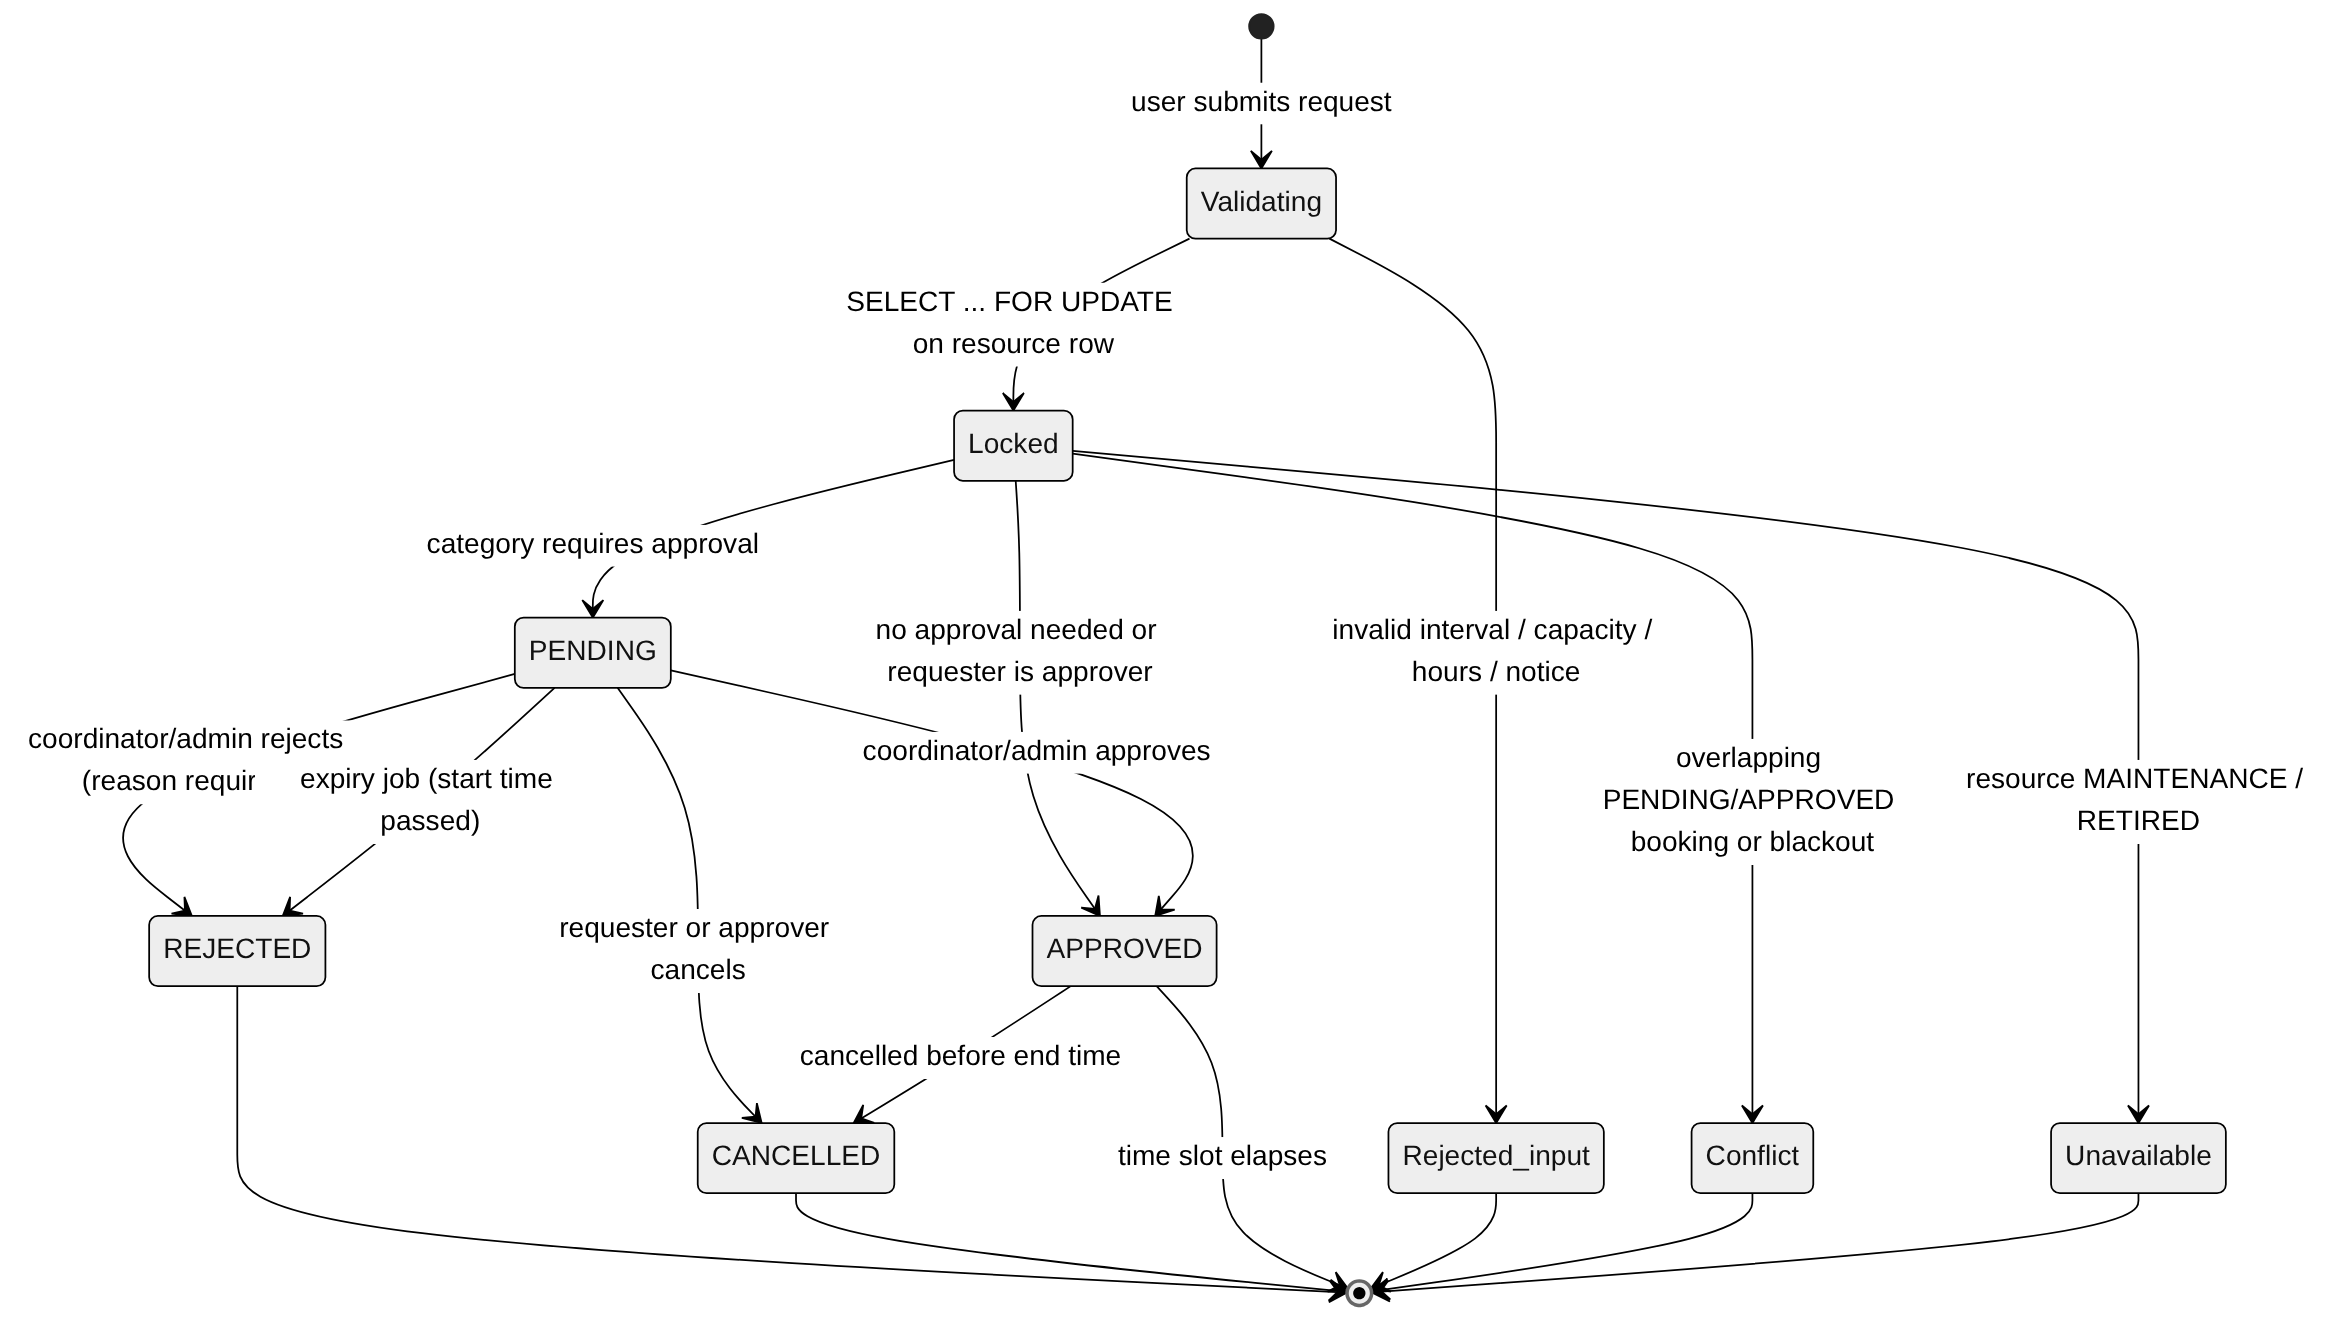
\includegraphics[width=\linewidth,height=0.55\textheight,keepaspectratio]{booking_workflow.png}
\caption{Booking life cycle enforced by sp\_create\_booking and trg\_bookings\_biu}\label{fig:workflow}
\end{figure}
\evidence{fig07_run_all.png}{run\_all.sql completing with ``All objects VALID''}
\evidence{fig08_objects_valid.png}{Verification V1--V2: every object VALID, no compilation errors}
\evidence{fig08_constraints.png}{Verification V4--V5: constraints per table; no unindexed foreign keys}
\evidence{fig10_two_sessions_naive.png}{Two-session naive check-then-insert and the resulting overlap query}

\chapter{Source Code}
The complete source code (all SQL scripts, the API and the front end) is in the submission archive and the project repository. The stored procedures and triggers --- the core of the concurrency and integrity design --- are reproduced in full below; the functions and package specifications are shown in Chapter~\ref{ch:impl}.

\lstset{basicstyle=\ttfamily\scriptsize\linespread{1.0}\selectfont}
\section{Stored procedures (06\_procedures.sql)}
\lstinputlisting[language=PLSQL]{../database/06_procedures.sql}
\section{Triggers (09\_triggers.sql)}
\lstinputlisting[language=PLSQL]{../database/09_triggers.sql}

\end{document}
